% !TEX root = thesis.tex
\chapter{Results and Evaluation}
\label{sec:results_and_evaluation}

This chapter evaluates the implemented \gls{snn} accelerator at both the hardware and application levels. It first verifies the correct operation of the processor--programmable-logic communication path, the accelerator interfaces, and the online weight-update mechanism. The implementation is then assessed in terms of \gls{fpga} resource utilization, timing performance, and end-to-end processing speed. Finally, the learning capability is evaluated using three complete training epochs on the MNIST dataset, followed by an analysis of classification accuracy, output activity, and class-dependent behaviour. The obtained results are compared with representative \gls{sdsp}-based hardware, with particular attention to TEDOP and to differences in neuron models, learning rules, data preparation, numerical precision, and measurement boundaries. The chapter concludes by discussing the significance and limitations of the results, particularly the use of a single-layer network and the limited number of training epochs.

\section{Experimental Setup and Evaluation Methodology}
\label{subsec:experimental-setup}

The evaluation was designed to separate three questions. First, the board-level tests determine whether the deployed accelerator accepts correctly formatted input transactions and exposes valid status and result information. Second, controlled learning tests determine whether teacher-guided \gls{sdsp} updates produce a persistent change in network behaviour. Third, complete MNIST training epochs assess whether these local updates improve classification performance over a larger workload. The following configuration and protocol were kept fixed so that changes observed between evaluations can be attributed to the learned synaptic state rather than to a change in the hardware or input representation.

\subsection{Hardware and Network Configuration}

All measurements use the final PYNQ-Z1 overlay described in Chapter \ref{sec:implementation}. The \gls{ps} loads the prepared spike data from storage, places one encoded image in a contiguous \gls{ddr} \gls{sdram} buffer, configures the accelerator through AXI4-Lite, and starts the memory-to-stream \gls{dma} transfer. The \gls{pl} receives the complete 100-step input sequence, executes the generated network schedule, performs local weight updates when learning is enabled, and records the output-neuron spike counts. Consequently, the reported board-level measurements include the complete implemented path rather than an isolated simulation of the learning rule.

The evaluated network contains 784 external inputs and ten \gls{lif} output neurons. No hidden layer is used. This configuration keeps the hardware experiment focused on the integration of online learning and provides the same input--output dimensions as the single-layer TEDOP network used later for comparison. The output spikes are also returned through the fixed inhibitory path to preserve the competition mechanism of the generated Spiker+ design. The topology choice and its implications for classification accuracy are discussed later in this chapter.

Table \ref{tab:evaluation-configuration} summarizes the configuration used throughout the board experiments. The teacher current is represented in the accelerator's fixed-point format. Its register value of 128 corresponds to 0.25 in Q9 representation. Calcium leakage is generated once every ten network time steps, while bistability events are disabled. These values were held constant across all three training epochs; the experiment therefore evaluates one defined hardware configuration rather than a parameter sweep.

\begin{table}[htbp]
	\centering
	\caption{Configuration Used for the Board-Level Evaluation}
	\label{tab:evaluation-configuration}
	\small
	\begin{tabularx}{\linewidth}{@{}p{0.32\linewidth}X@{}}
		\toprule
		\textbf{Item} & \textbf{Evaluation configuration} \\
		\midrule
		Target platform & PYNQ-Z1 with an XC7Z020 device \\
		Programmable-logic clock & 100\,MHz \\
		Network topology & 784 external inputs and ten output neurons, without a hidden layer \\
		Neuron model & Modified subtractive-reset \gls{lif} neuron with recurrent output inhibition \\
		Input duration & 100 network time steps per image \\
		Spike encoding & Rate coding using the Spiker+ MNIST data loader with a gain of 0.1 \\
		Input transaction & 25 32-bit words per time step; 2,500 words or 10,000 bytes per image \\
		Excitatory weights & 3-bit unsigned weights stored as a 784-by-30-bit memory \\
		Learning mode & Teacher-guided \gls{sdsp} enabled during training and disabled during evaluation \\
		Teacher current & Register value 128, corresponding to 0.25 in Q9 representation \\
		Calcium leakage & One leak event every ten network time steps \\
		Bistability & Disabled \\
		Output decision & Index of the output neuron with the largest spike count \\
		\bottomrule
	\end{tabularx}
\end{table}

\subsection{Dataset Preparation and Experimental Protocol}

The application-level evaluation uses the MNIST handwritten-digit dataset, which provides separate training and test partitions \cite{LeCun1998GradientBasedLearning}. The complete set of 60,000 training images is presented once in each epoch. To retain the stochastic behaviour of rate coding, the image order and the generated spike realization are produced independently for every epoch. Seeds 2028, 2029, and 2030 are used for epochs one to three, respectively. Each resulting archive contains 60 ordered shards of 1,000 images. The archive manifest records the encoding parameters, label distribution, and input-spike count, while a SHA-256 digest is checked after transfer to the board. This prevents an incomplete or different archive from being used unnoticed.

A separate class-balanced subset of 1,000 images is selected from the MNIST test partition using seed 2027. It contains 100 images from each digit class and excludes the first ten test images that had previously been used for small functional checks. Unlike the training inputs, this set is encoded only once and stored as a fixed spike archive. Reusing the identical packed words before training and after every epoch removes stochastic re-encoding as a cause of differences between evaluation points.

Figure \ref{fig:evaluation-protocol} shows the resulting experimental sequence. The bitstream is first loaded once to restore the initial weights, after which a baseline evaluation is performed. Training and evaluation then alternate for three epochs. Learning and teacher input are enabled only for the 60,000 training transactions of an epoch. Both are disabled when the fixed 1,000-image set is evaluated. The FPGA is not reprogrammed between epochs, because doing so would restore the initialized weight memory and discard the learning achieved by the preceding epoch. A soft reset before an image clears the transaction and neural state required for a new sample without replacing the learned synaptic weights.

\begin{figure}[t]
	\centering
	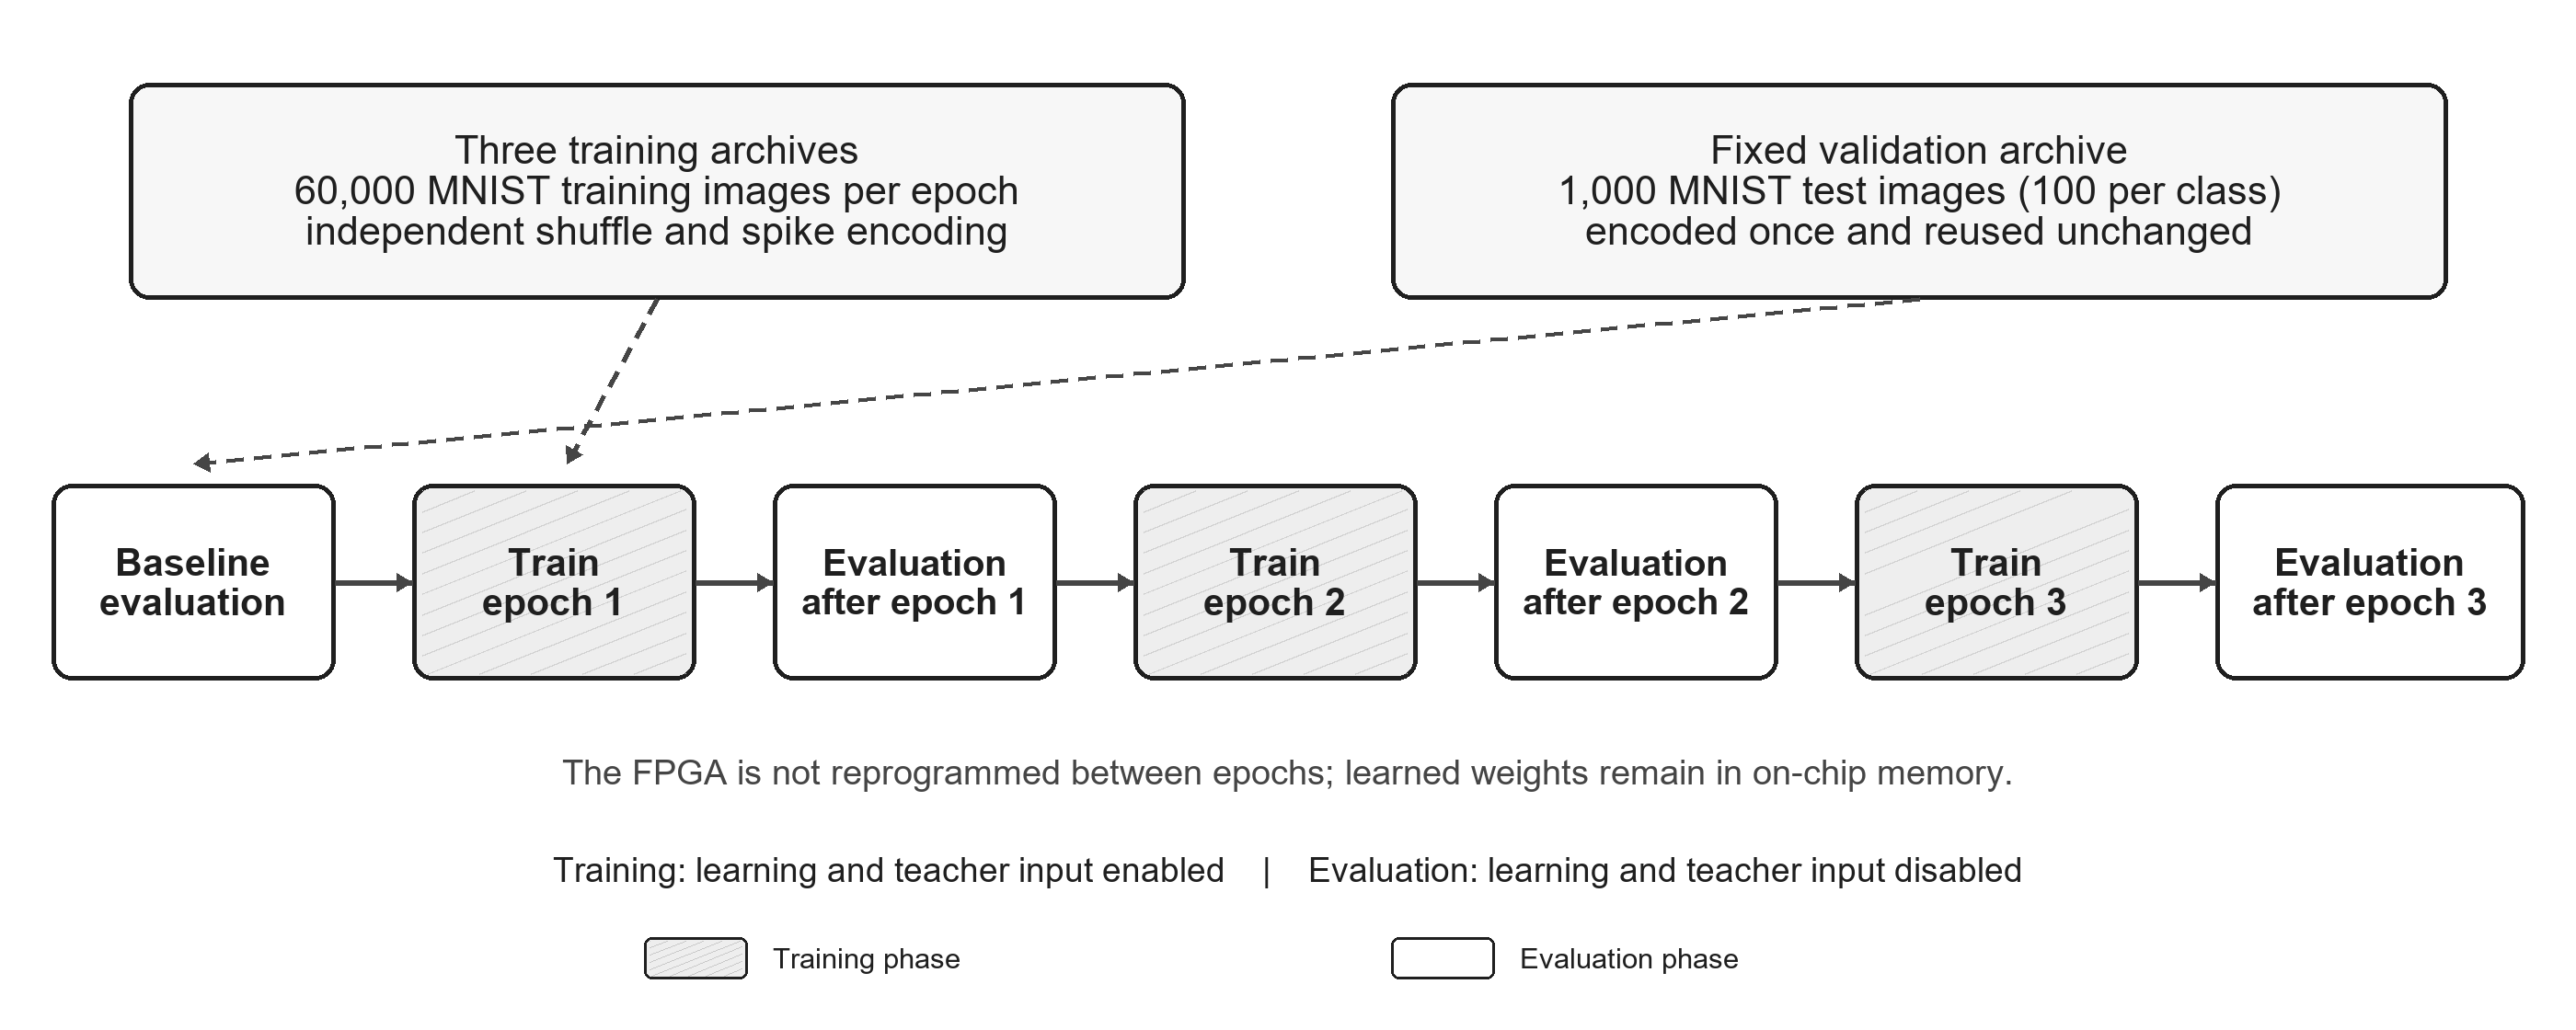
\includegraphics[width=\linewidth]{figures/evaluation_protocol.png}
	\caption{Training and Evaluation Protocol Used for the Three-Epoch Board Experiment}
	\label{fig:evaluation-protocol}
\end{figure}

Although the fixed images originate from the MNIST test partition, they are referred to as the \emph{validation set} in this chapter. Their results were inspected after each epoch and used to decide whether an additional epoch should be run. They therefore participated indirectly in the experimental decision process and do not constitute a fully independent final test set. This distinction limits the claims that can be made from the measured accuracy and is considered again in the discussion of the results.

\subsection{Evaluation Metrics}

Classification is derived from the ten output-neuron spike counts accumulated over one 100-step transaction. A sample is defined as \emph{silent} when all ten counts are zero. Silent samples require explicit treatment because applying a numerical argmax operation to an all-zero vector returns the first class even though the network produced no classification evidence. The primary metric is therefore strict accuracy, for which every silent sample is counted as incorrect.

Table \ref{tab:evaluation-metrics} defines the metrics reported in the following sections. Active-image accuracy is included as a diagnostic measure rather than as an alternative overall accuracy. Comparing it with strict accuracy reveals whether an improvement results from better class separation among responding samples or merely from a reduction in the number of silent samples. Total output spikes and the class-wise results provide complementary information about changes in network activity that would not be visible from accuracy alone.

\begin{table}[htbp]
	\centering
	\caption{Metrics Used to Evaluate the Online-Learning Experiment}
	\label{tab:evaluation-metrics}
	\small
	\begin{tabularx}{\linewidth}{@{}p{0.25\linewidth}X@{}}
		\toprule
		\textbf{Metric} & \textbf{Definition and purpose} \\
		\midrule
		Strict accuracy & Fraction of all validation images for which at least one output spike is produced and the neuron with the largest count corresponds to the true class. Silent images are counted as incorrect. \\
		Raw argmax accuracy & Fraction obtained by applying argmax directly to every count vector. This value is reported only as a diagnostic because an all-zero vector is assigned to class zero. \\
		Active-image accuracy & Accuracy calculated only over images that produce at least one output spike. It separates classification behaviour from the silent-output problem. \\
		Silent images & Number of images for which the sum of all ten output spike counts is zero. \\
		Total output spikes & Sum of all output-neuron spike counts over the complete validation set, used to characterize overall network activity. \\
		Per-class accuracy & Strict accuracy calculated separately for each digit class, used to identify class-dependent learning behaviour. \\
		\bottomrule
	\end{tabularx}
\end{table}

The reported learning curve is obtained from one continuous three-epoch hardware run. The independently encoded training archives introduce new spike realizations between epochs, whereas the fixed validation archive makes the four evaluation points directly comparable. However, the experiment does not include repeated training runs with different initial weights or parameter combinations. The results therefore demonstrate the behaviour and learning trend of the implemented configuration, but they do not provide an estimate of statistical variation across independent runs.

\section{Hardware Functional Validation}
\label{subsec:hardware-functional-validation}

Before evaluating classification performance, the deployed system was tested to establish that input data, control values, neural activity, and learning operations pass through the intended hardware path. These tests were performed on the PYNQ-Z1 using the final bitstream and its matching hardware-description file. They complement the RTL verification described in Section \ref{subsec:verification-infrastructure}: simulation checks internal timing and interface contracts, whereas the experiments in this section verify the integrated \gls{ps}, \gls{dma}, AXI, and accelerator system on the physical board.

\subsection{Board-Level Interface and Data-Path Tests}

The first checks were deliberately independent of MNIST classification accuracy. The overlay metadata was parsed before configuration to confirm that the memory-to-stream \gls{dma} and accelerator control interface appeared at the expected addresses. After configuration, the AXI4-Lite registers reported an idle accelerator, 100 configured time steps, and disabled learning and teacher modes. Configuration values written by the processor, including the target label, calcium-leak interval, bistability interval, and teacher current, were subsequently read back before an input transaction was started.

Two deterministic edge cases were then used to make failures directly observable. The zero-input test sent 100 time steps without an input spike. All steps were accepted, no stream or \gls{dma} error was reported, and the ten output-neuron counts remained zero. The dense-input test asserted all 784 valid input bits at every time step while keeping the unused upper bits of the final stream word at zero. The accelerator again accepted all 100 steps and reported 99 spikes for each output neuron, matching the behaviour observed in the corresponding RTL test. These cases exercise both inactivity and sustained input activity without depending on a trained classifier.

Table \ref{tab:board-functional-tests} summarizes the board-level checks. The fixed MNIST frames additionally verified that the packed 25-word representation could be transferred repeatedly and that the output counters could be read after each completed transaction. Finally, a 1,000-image supervised pilot completed without a transfer timeout, malformed-stream indication, or incomplete input count. Passing this test establishes continuous operation of the integrated data and control paths; it does not by itself establish that the resulting classifier is accurate.

\begin{table}[htbp]
	\centering
	\caption{Summary of Board-Level Functional Tests}
	\label{tab:board-functional-tests}
	\small
	\begin{tabularx}{\linewidth}{@{}p{0.20\linewidth}p{0.33\linewidth}X@{}}
		\toprule
		\textbf{Test} & \textbf{Applied check} & \textbf{Board observation} \\
		\midrule
		Overlay metadata & Parse the hardware description and inspect the instantiated IP blocks & The MM2S \gls{dma} and accelerator interfaces were present at their expected AXI addresses. \\
		Register interface & Read defaults, write the runtime parameters, and read them back & The accelerator reported 100 time steps and retained the programmed learning parameters. \\
		Zero-input stream & Transfer 2,500 zero-valued words with learning and teacher input disabled & All 100 steps were accepted, no interface error was set, and all ten output counts remained zero. \\
		Dense-input stream & Assert all 784 valid input bits in every time step & All 100 steps were accepted and every output neuron produced 99 spikes, consistent with RTL verification. \\
		MNIST inference & Transfer fixed, pre-encoded MNIST frames without learning & Each transaction completed with 100 accepted steps and reproducible output-count vectors. \\
		Teacher path & Train one label-7 sample with a Q9 teacher current of 128 & Only the selected output neuron responded to the teacher current, producing 27 spikes in the initial directed test. \\
		Continuous training & Process 1,000 supervised MNIST training images without reconfiguration & All images completed without a \gls{dma} timeout, stream error, or incomplete step count. \\
		\bottomrule
	\end{tabularx}
\end{table}

\subsection{Controlled Teacher-Signal and Weight-Update Test}

Activity observed while the teacher current is applied cannot alone prove that synaptic weights were updated. The additional current can directly cause the selected neuron to spike even if the new weight value is not stored. A controlled experiment was therefore performed to determine whether teacher-guided training leaves a persistent effect after both learning and teacher input have been disabled.

Figure \ref{fig:teacher-control-validation} shows the experiment and its observations. Both branches start by reloading the same bitstream and recording the initial inference counts of ten fixed MNIST samples. In the teacher-off control branch, sample zero, whose label is seven, is presented ten times with learning enabled but teacher input disabled. A subsequent inference pass over the ten samples produces exactly the same count vectors as the initial baseline. In the teacher-enabled branch, the initial weights are restored again and the same sample is presented for the same number of repetitions, this time with the label-7 teacher input enabled. During the following inference pass, five of the ten samples differ from the teacher-off result. Every observed difference is confined to output neuron seven, which is the neuron selected by the training label.

\begin{figure}[t]
	\centering
	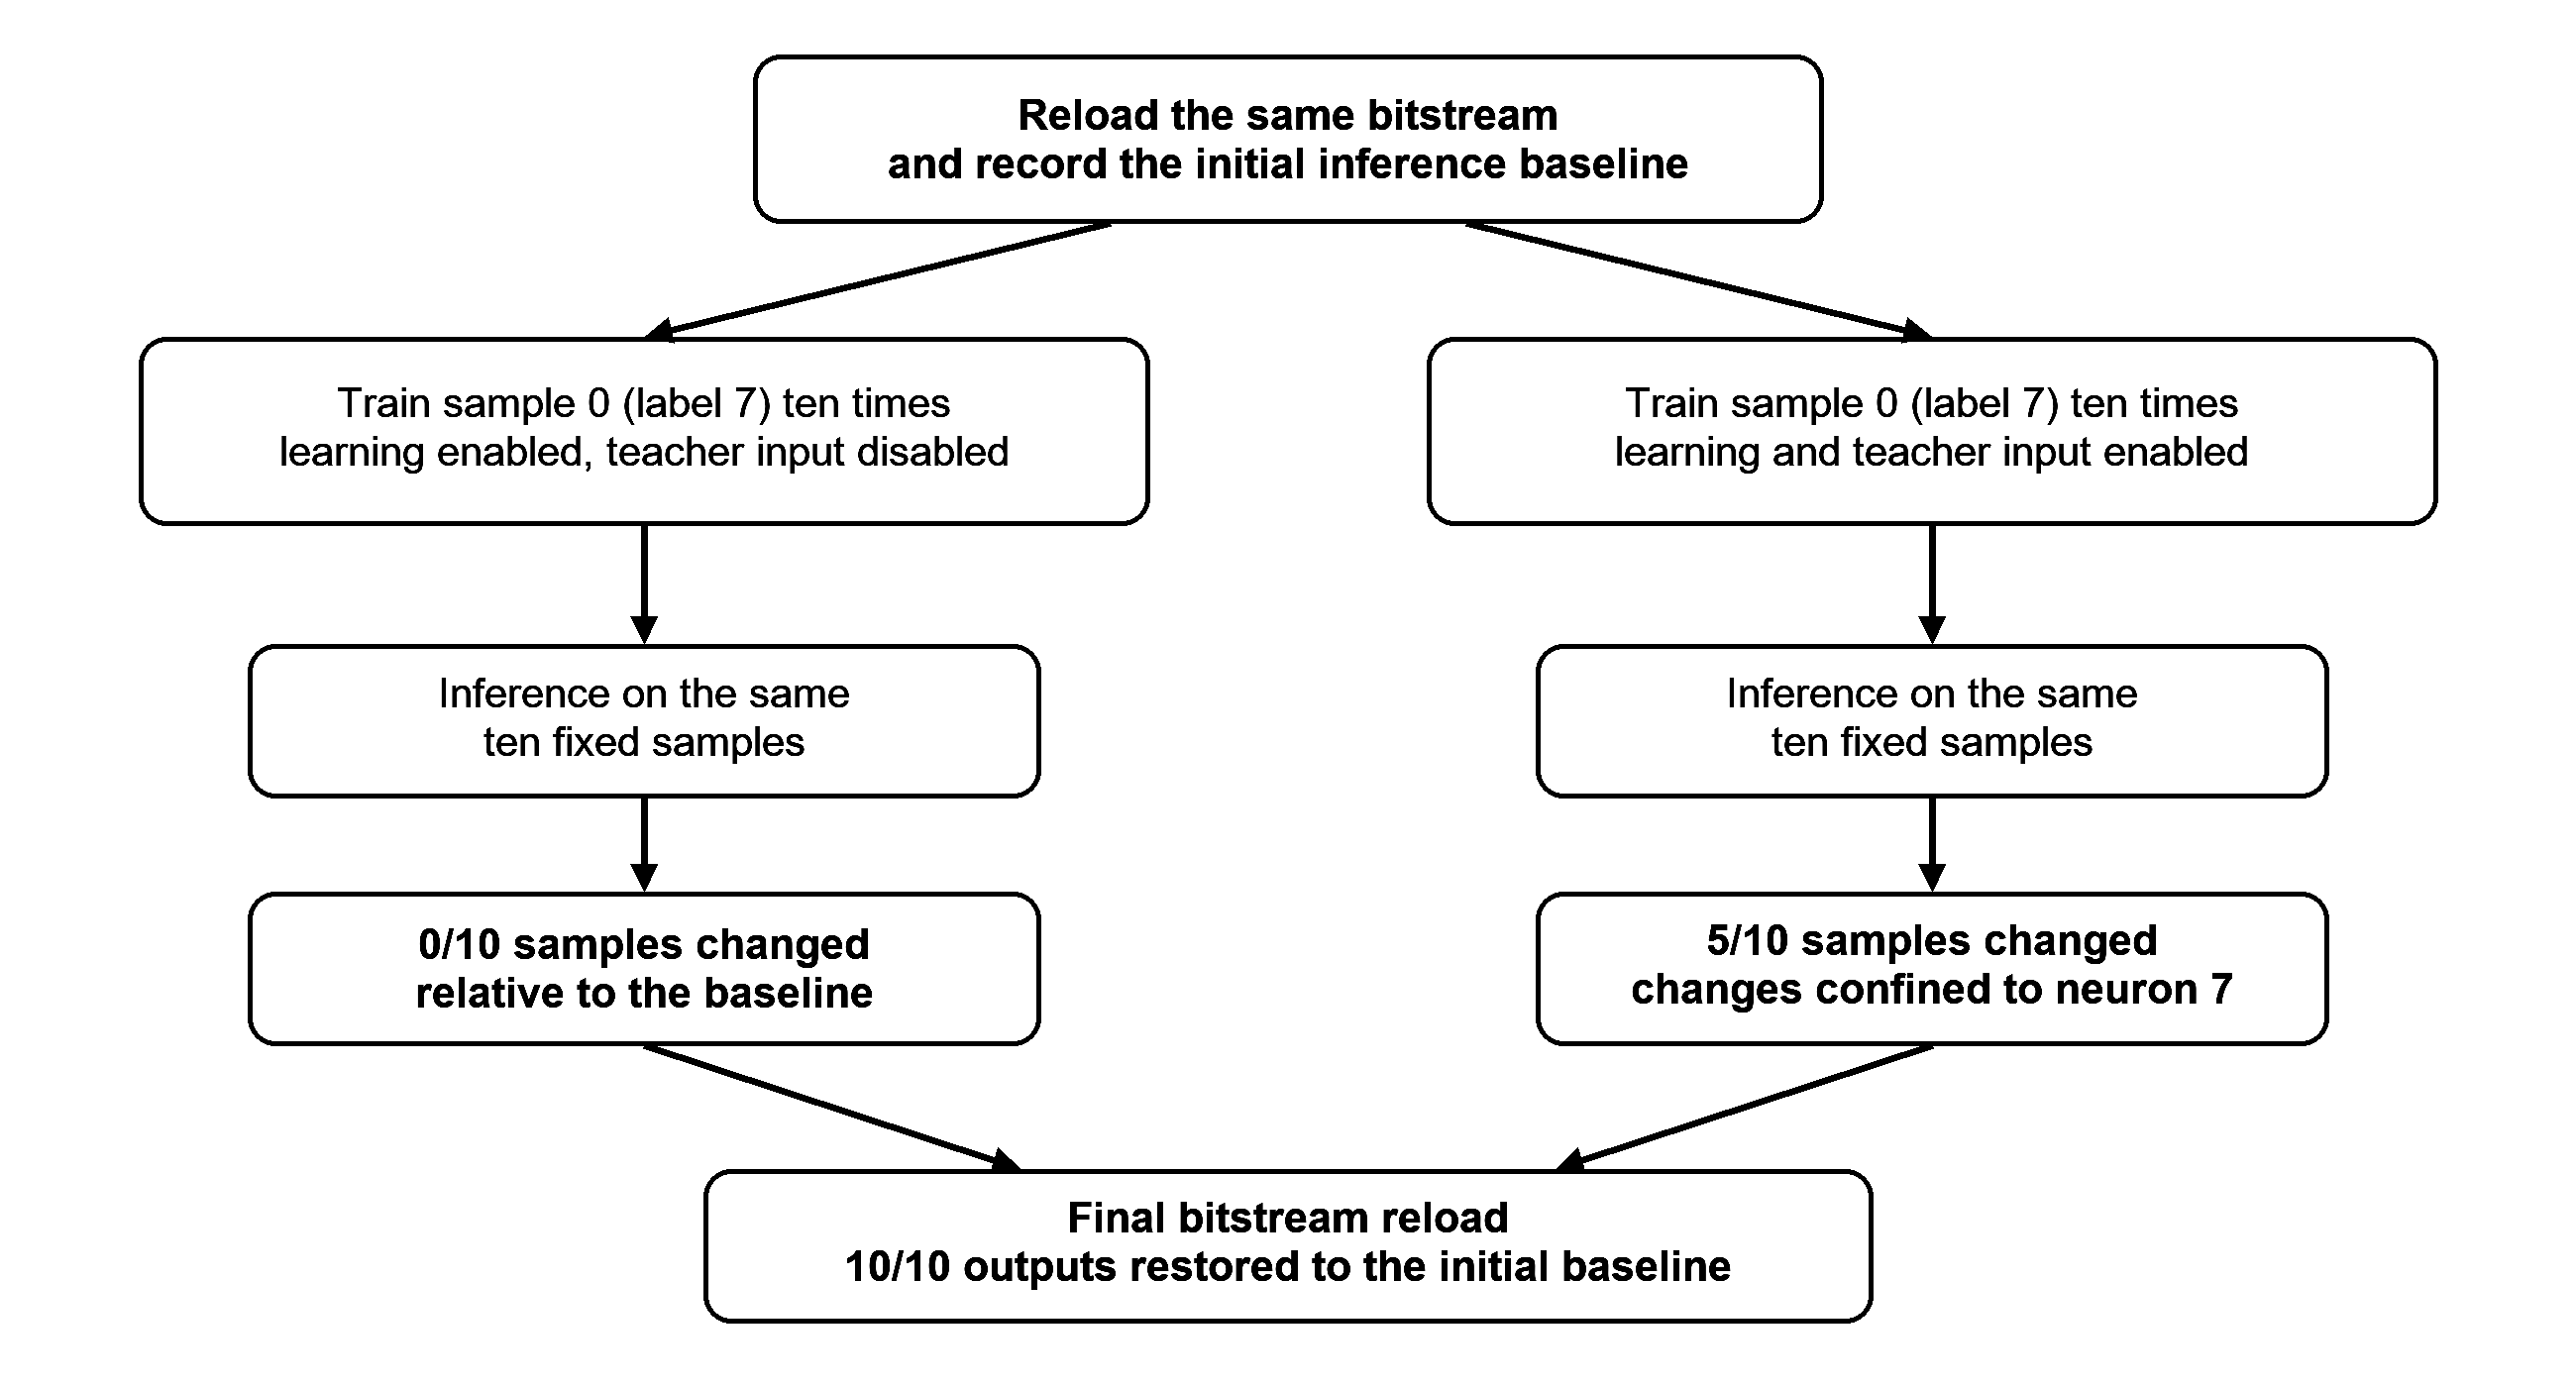
\includegraphics[width=\linewidth]{figures/teacher_control_validation.png}
	\caption{Teacher-Input Control Experiment and Observed Output Changes}
	\label{fig:teacher-control-validation}
\end{figure}

The inference transactions include a soft reset that clears the state required to start a new image while retaining the contents of the weight memory. The changed response therefore persists beyond the training transaction and cannot be explained only by the teacher current remaining active. As a final control, the bitstream is reloaded after the teacher-enabled experiment. All ten inference outputs then return to the recorded initial baseline. This confirms that the changed behaviour is associated with state stored in the configured accelerator and is discarded when the weight memory is reinitialized.

Taken together, the teacher-off branch, the target-specific change after teacher-enabled training, and restoration after bitstream reload provide behavioural evidence that the teacher path affects persistent synaptic updates. The experiment does not constitute a direct read-back of individual weight values because the implemented software interface exposes spike counts but not the complete excitatory memory. The conclusion is therefore limited to an observable and repeatable change in network behaviour consistent with the intended weight-update path.

\subsection{Software--Hardware Behavioural Comparison}

A final diagnostic test compares the deployed accelerator with the Spiker+ software model using the same stored input words. The first comparison exposed a difference in the initial conditions: the default software model initialized all excitatory weights with codes one and two, whereas the generated RTL initialization contains values across the complete 3-bit range. With these different weights, the software model remained silent for all ten samples while the hardware produced 176 output spikes. This result demonstrates why common input data alone are insufficient for a meaningful parity comparison.

The RTL initialization package was therefore decoded and loaded into the software model before repeating the baseline. Table \ref{tab:software-hardware-comparison} gives the resulting comparison and the measurements after both implementations processed the same 1,000-image training archive. With aligned initial weights, both models contain four silent samples and their total output activity differs by only 15 spikes before training. Five of the ten complete output-count vectors agree exactly. Following the training pilot, total activity decreases in both implementations, although the hardware exhibits a stronger reduction.

\begin{table}[htbp]
	\centering
	\caption{Software--Hardware Comparison on Ten Preserved MNIST Inputs}
	\label{tab:software-hardware-comparison}
	\small
	\begin{tabularx}{\linewidth}{@{}X >{\centering\arraybackslash}p{0.15\linewidth} >{\centering\arraybackslash}p{0.13\linewidth} >{\centering\arraybackslash}p{0.12\linewidth} >{\centering\arraybackslash}p{0.16\linewidth}@{}}
		\toprule
		\textbf{Comparison condition} & \textbf{Total spikes SW/HW} & \textbf{Silent SW/HW} & \textbf{Exact vectors} & \textbf{Absolute difference} \\
		\midrule
		Spiker+ default-weight baseline & 0/176 & 10/4 & 4/10 & 176 \\
		RTL-initialized baseline & 161/176 & 4/4 & 5/10 & 15 \\
		After the 1,000-image pilot & 42/20 & 4/6 & 4/10 & 26 \\
		\bottomrule
	\end{tabularx}
\end{table}

The post-training reduction is consequently not a hardware-only anomaly: the software model shows the same direction of change when it uses the preserved inputs and RTL-derived initial weights. Nevertheless, the two implementations are not bit-exact. The software model evaluates neuron dynamics with floating-point operations, whereas the accelerator uses fixed-point arithmetic, integer shifts, and an explicit multi-cycle schedule. These numerical and timing differences provide plausible sources for the remaining count deviations, but the present experiment does not isolate their individual contributions. The comparison therefore supports agreement at the behavioural-trend level rather than cycle-accurate equivalence.

Overall, the board tests verify the complete input and control path, isolate the effect of teacher-guided learning, and demonstrate that weight-dependent behaviour persists across transactions. These observations establish the functional basis required for the larger resource, performance, and three-epoch learning evaluations presented in the following sections.

\section{FPGA Implementation Results}
\label{subsec:fpga-implementation-results}

The final block design was synthesized, placed, and routed for the XC7Z020 device on the PYNQ-Z1. The results in this section are taken from the Vivado post-implementation reports and therefore describe the complete programmable-logic design, including the SNN accelerator IP and the supporting AXI, DMA, interconnect, and buffering logic introduced in Chapter~\ref{sec:implementation}. They should not be interpreted as measurements of the learning module in isolation.

\subsection{Resource Utilization}

Table~\ref{tab:implementation-resource-utilization} lists the implemented resource usage. LUTs are the most heavily used resource, with 5,056 of the 53,200 available LUTs occupied, corresponding to 9.50\%. The design uses 5,294 flip-flops, or 4.98\% of the device capacity. LUTRAM, BRAM, and global clock-buffer usage all remain below 3.2\%. The same percentages are visualized in Figure~\ref{fig:implementation-results-summary}.

\begin{table}[htbp]
	\centering
	\caption{Post-Implementation Resource Utilization on the XC7Z020}
	\label{tab:implementation-resource-utilization}
	\small
	\begin{tabular}{@{}lrrr@{}}
		\toprule
		\textbf{Resource} & \textbf{Used} & \textbf{Available} & \textbf{Utilization} \\
		\midrule
		LUT    & 5,056 & 53,200  & 9.50\% \\
		LUTRAM & 138   & 17,400  & 0.79\% \\
		FF     & 5,294 & 106,400 & 4.98\% \\
		BRAM   & 4     & 140     & 2.86\% \\
		BUFG   & 1     & 32      & 3.13\% \\
		\bottomrule
	\end{tabular}
\end{table}

The low overall percentages show that the integrated design fits comfortably on the selected device and leaves substantial programmable-logic capacity unused. This headroom could support additional control logic or a larger accelerator configuration. However, the percentages alone do not establish how far the network can be scaled: weight-memory capacity, memory bandwidth, and the sequential layer schedule must also be considered.

\begin{figure}[t]
	\centering
	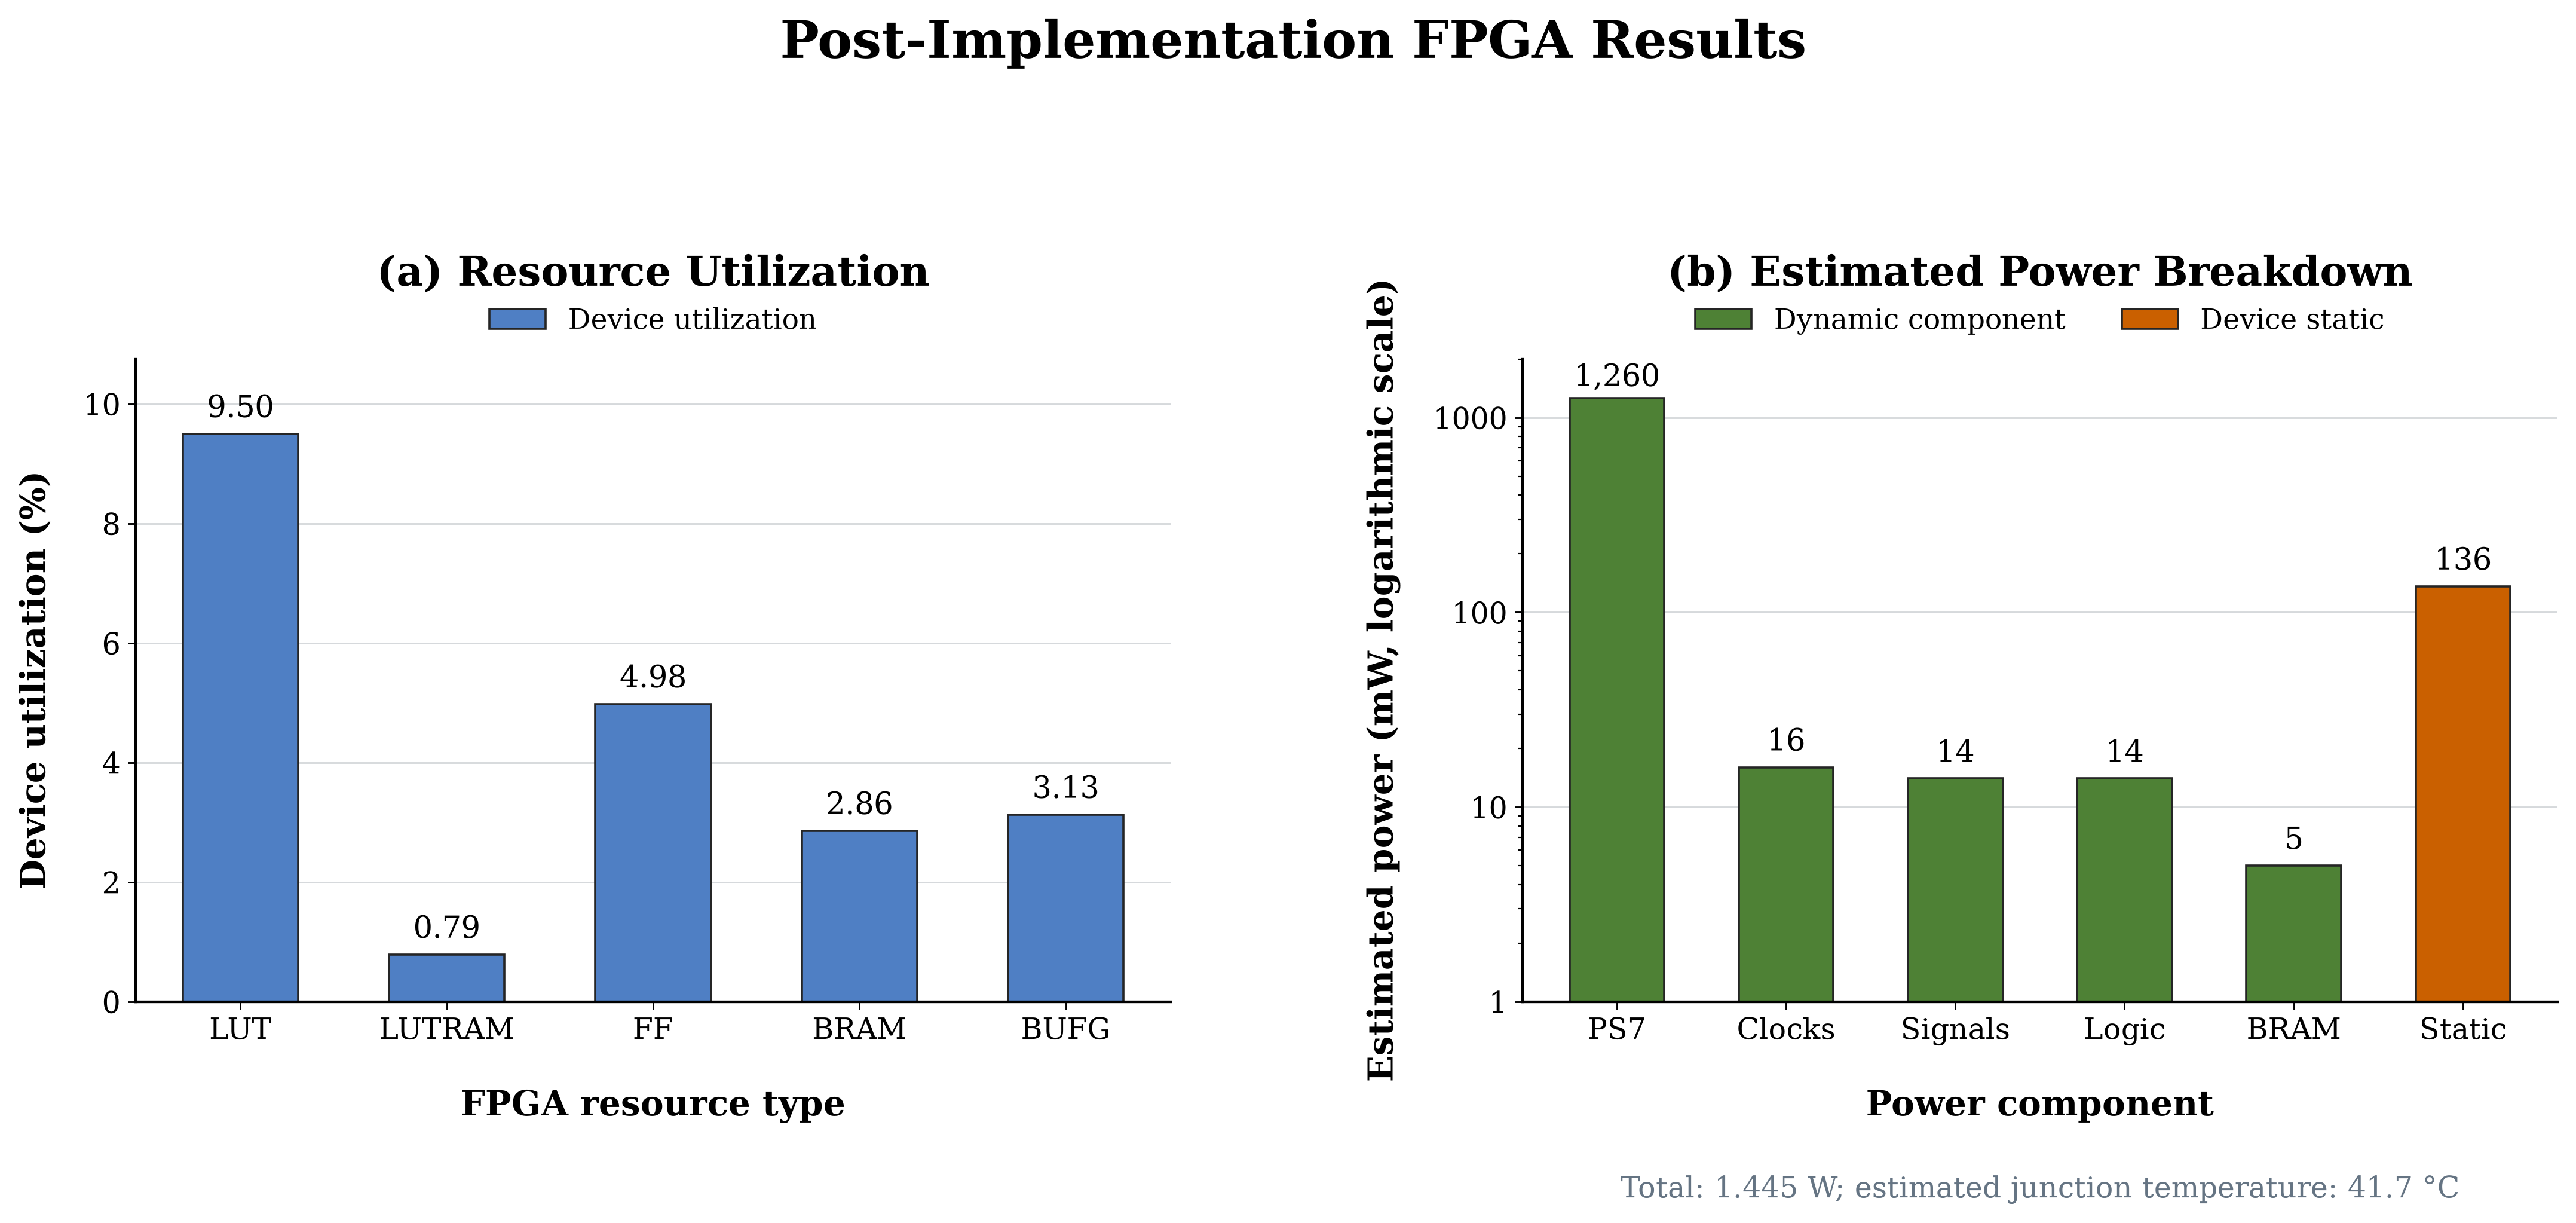
\includegraphics[width=\linewidth]{figures/implementation_results_summary.png}
	\caption{Post-Implementation Resource Utilization and Vivado Power Estimate for the Complete PYNQ-Z1 Design}
	\label{fig:implementation-results-summary}
\end{figure}

\subsection{Power and Thermal Estimate}

Table \ref{tab:implementation-power-summary} records the principal power and thermal values from the post-implementation report. Vivado estimates a total on-chip power of 1.445~W, divided into 1.309~W of dynamic power and 0.136~W of static power. Dynamic power therefore represents approximately 91\% of the estimate. Within the reported dynamic-power breakdown, the PS7 accounts for 1.260~W, or approximately 96.3\% of dynamic power. The reported contributions from clocks, signals, logic, and BRAM are 0.016~W, 0.014~W, 0.014~W, and 0.005~W, respectively. These four non-PS categories sum to approximately 49~mW, but they cover the complete programmable-logic design and cannot be attributed exclusively to the SNN accelerator.

\begin{table}[htbp]
	\centering
	\caption{Vivado Post-Implementation Power and Thermal Summary}
	\label{tab:implementation-power-summary}
	\small
	\begin{tabularx}{\linewidth}{@{}Xr@{}}
		\toprule
		\textbf{Reported quantity} & \textbf{Value} \\
		\midrule
		Total on-chip power & 1.445~W \\
		Dynamic power & 1.309~W (91\%) \\
		Static power & 0.136~W (9\%) \\
		Estimated junction temperature & 41.7~$^{\circ}$C \\
		Thermal margin & 43.3~$^{\circ}$C (3.6~W) \\
		Effective $\theta_{JA}$ & 11.5~$^{\circ}$C/W \\
		Power supplied to off-chip devices & 0~W \\
		Report confidence level & Medium \\
		\bottomrule
	\end{tabularx}
\end{table}

The estimated junction temperature is 41.7~$^{\circ}$C and the reported thermal margin is 43.3~$^{\circ}$C, indicating that the implemented configuration is not thermally constrained under the assumptions used by Vivado. Nevertheless, this result is an implementation estimate with a medium confidence level, not a measurement at the board power input. Moreover, it includes the processing system and the surrounding programmable-logic infrastructure. It is therefore unsuitable for a direct power-efficiency comparison with accelerator-only measurements reported by other neuromorphic processors unless a common measurement boundary and workload are established.

\subsection{Timing Closure}

Timing was evaluated for the implemented 100~MHz design. Table~\ref{tab:implementation-timing-summary} records the setup, hold, and pulse-width results. All three worst-case slack values are positive, the total negative slack is zero, and Vivado reports no failing endpoints. The smallest margin is the 0.012~ns worst hold slack, but it remains positive after implementation.

\begin{table}[htbp]
	\centering
	\caption{Post-Implementation Timing Summary at 100~MHz}
	\label{tab:implementation-timing-summary}
	\small
	\begin{tabularx}{\linewidth}{@{}X >{\centering\arraybackslash}p{0.16\linewidth} >{\centering\arraybackslash}p{0.20\linewidth} >{\centering\arraybackslash}p{0.16\linewidth} >{\centering\arraybackslash}p{0.12\linewidth}@{}}
		\toprule
		\textbf{Check} & \textbf{Worst slack} & \textbf{Total negative slack} & \textbf{Failing endpoints} & \textbf{Endpoints} \\
		\midrule
		Setup       & 0.117~ns & 0~ns & 0 & 16,053 \\
		Hold        & 0.012~ns & 0~ns & 0 & 16,053 \\
		Pulse width & 3.750~ns & 0~ns & 0 & 5,565 \\
		\bottomrule
	\end{tabularx}
\end{table}

These results demonstrate timing closure at the configured 100~MHz operating frequency for the final routed design. The positive setup slack should not be treated as a measured maximum clock frequency; determining such a limit would require progressively tightening the clock constraint and repeating implementation. Together with the resource and power reports, the timing results establish that the complete integrated system is implementable on the PYNQ-Z1 with substantial resource headroom and without reported timing violations at the selected operating point.

\section{Runtime Performance}
\label{subsec:runtime-performance}

Runtime was measured at the Python application boundary on the PYNQ-Z1. One image corresponds to a complete accelerator transaction containing 100 network time steps and 25 32-bit stream words per step. The reported wall times therefore include the interaction between the processing system and programmable logic rather than only the execution time of the SNN core.

\subsection{End-to-End Processing Time}

The fixed 1,000-image validation set was evaluated four times: once with the initial weights and once after each training epoch. Learning and teacher input were disabled during these measurements. As shown in Table~\ref{tab:runtime-performance}, all four evaluations took between 14.73~s and 14.80~s. Across the 4,000 inference transactions, the mean time was 14.76~ms per image, corresponding to an end-to-end throughput of approximately 67.8 images/s.

Each complete training epoch presented 60,000 images with learning and the label-dependent teacher input enabled. Epochs one, two, and three required 905.02~s, 910.33~s, and 905.42~s, respectively. Their corresponding throughputs are 66.30, 65.91, and 66.27 images/s. The three epochs processed 180,000 training images in a total of 2,720.77~s, or 45~min 20.77~s, yielding an aggregate throughput of 66.16 images/s. Figure~\ref{fig:runtime-performance} visualizes the measured consistency across the complete experiment.

\begin{table}[htbp]
	\centering
	\caption{Measured End-to-End Runtime on the PYNQ-Z1}
	\label{tab:runtime-performance}
	\small
	\begin{tabularx}{\linewidth}{@{}X >{\centering\arraybackslash}p{0.12\linewidth} >{\centering\arraybackslash}p{0.16\linewidth} >{\centering\arraybackslash}p{0.16\linewidth} >{\centering\arraybackslash}p{0.15\linewidth}@{}}
		\toprule
		\textbf{Measurement} & \textbf{Images} & \textbf{Wall time} & \textbf{Mean time/image} & \textbf{Throughput} \\
		\midrule
		Initial-weight evaluation & 1,000 & 14.80~s & 14.80~ms & 67.57 images/s \\
		Evaluation after epoch 1 & 1,000 & 14.73~s & 14.73~ms & 67.89 images/s \\
		Evaluation after epoch 2 & 1,000 & 14.73~s & 14.73~ms & 67.89 images/s \\
		Evaluation after epoch 3 & 1,000 & 14.76~s & 14.76~ms & 67.75 images/s \\
		Training epoch 1 & 60,000 & 905.02~s & 15.08~ms & 66.30 images/s \\
		Training epoch 2 & 60,000 & 910.33~s & 15.17~ms & 65.91 images/s \\
		Training epoch 3 & 60,000 & 905.42~s & 15.09~ms & 66.27 images/s \\
		\bottomrule
	\end{tabularx}
\end{table}

\begin{figure}[t]
	\centering
	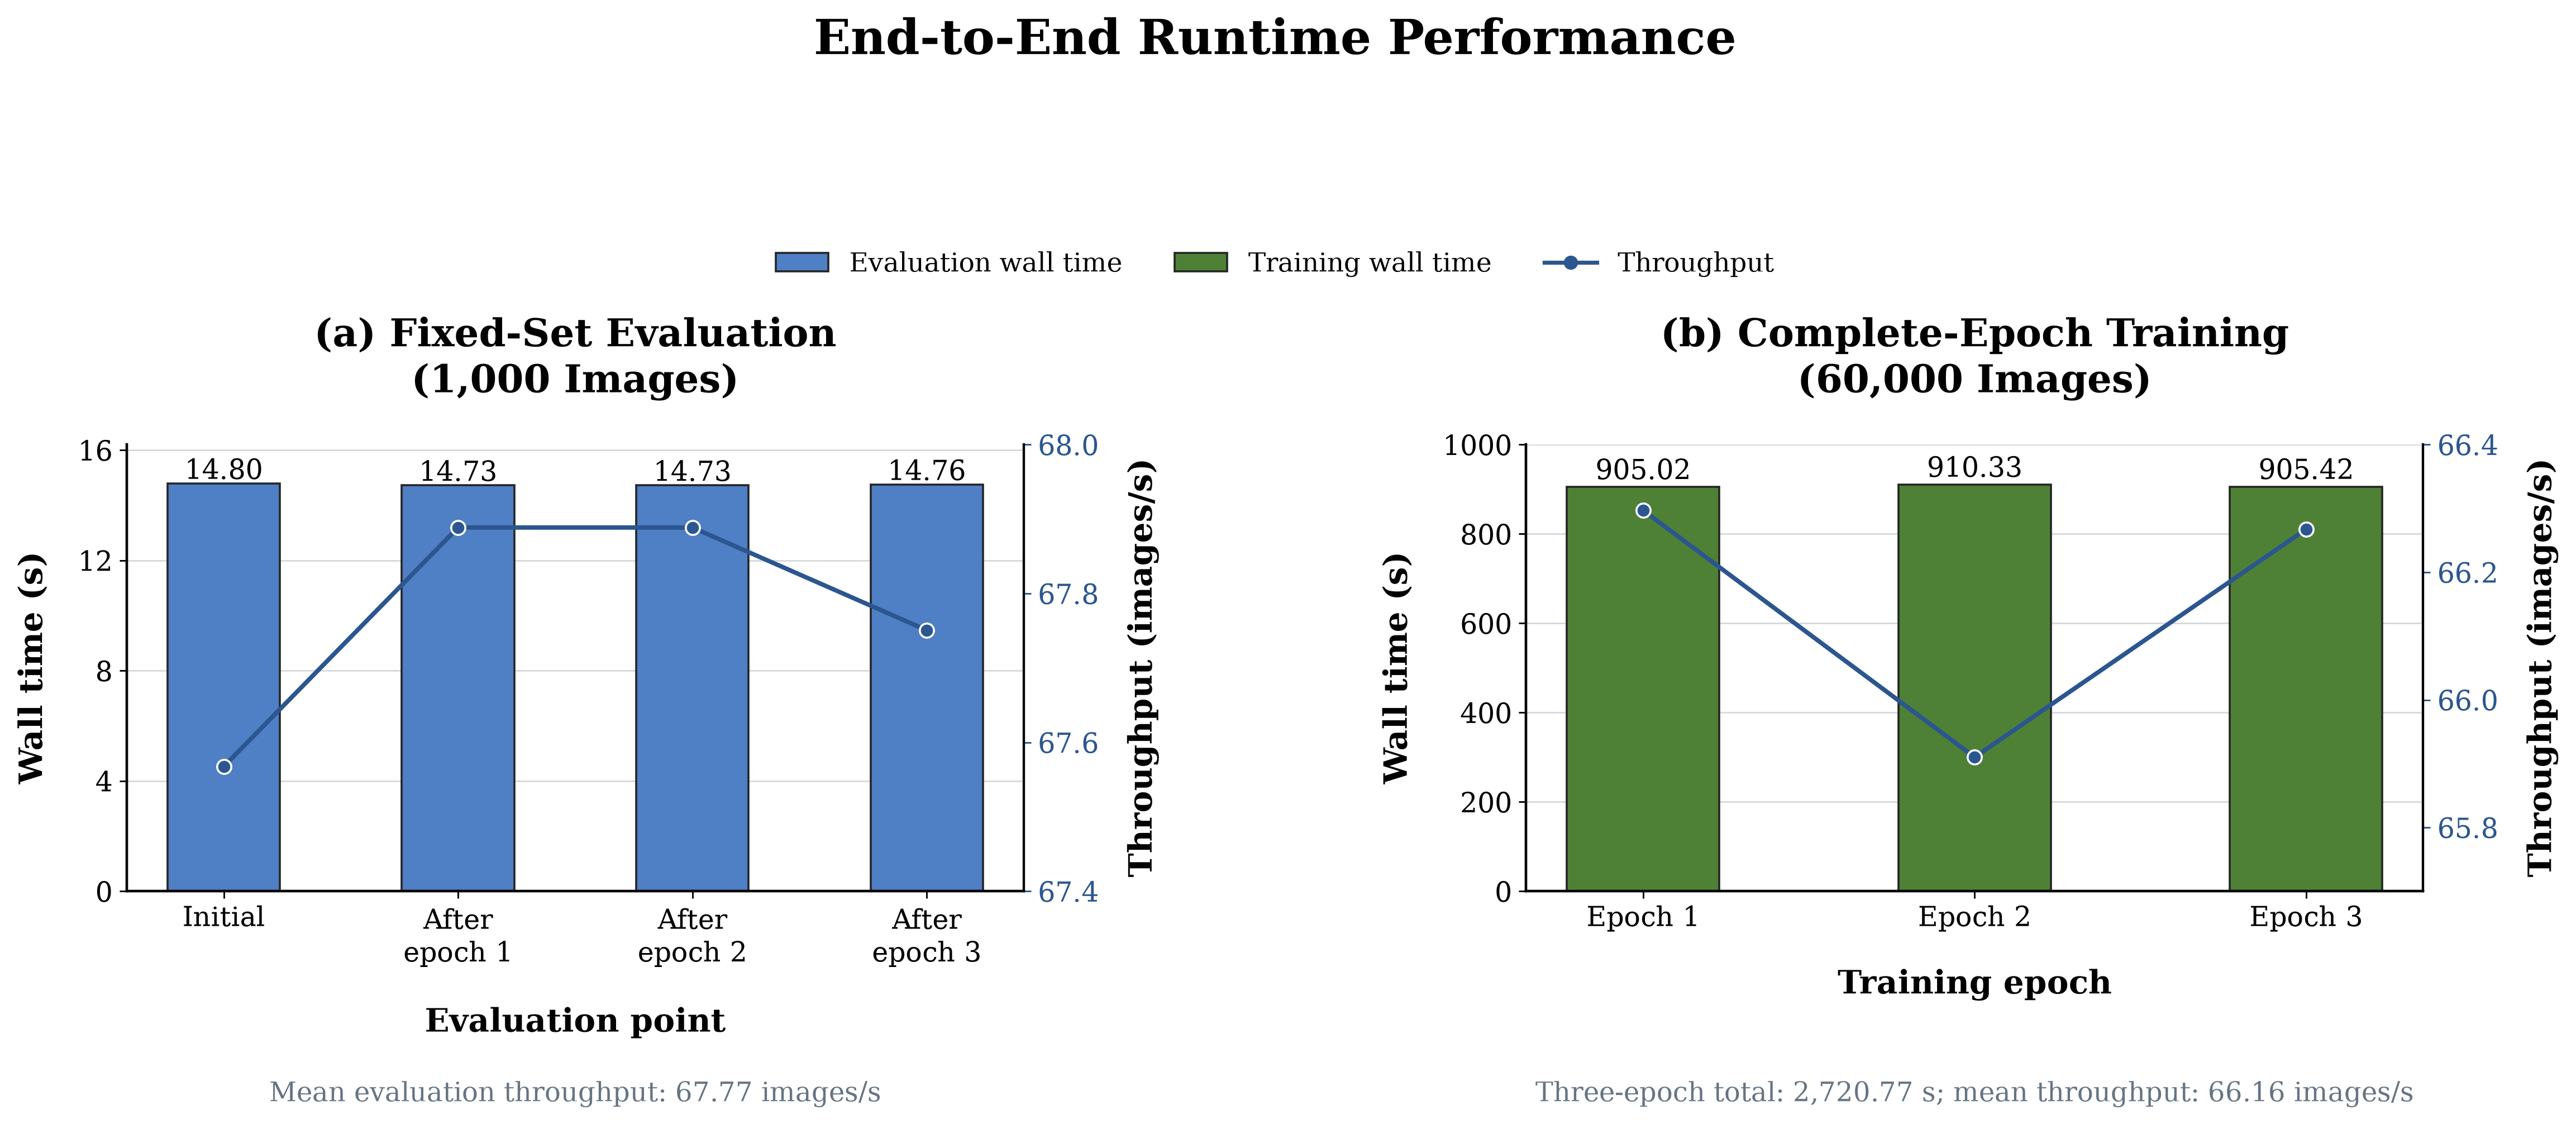
\includegraphics[width=\linewidth]{figures/runtime_performance.png}
	\caption{Measured End-to-End Runtime and Throughput for Evaluation and Training on the PYNQ-Z1}
	\label{fig:runtime-performance}
\end{figure}

The small variation between repeated validation measurements shows that the transaction time is stable as the synaptic weights and output activity change. Training is only slightly slower at the application level: the mean training time is 15.12~ms per image, compared with 14.76~ms for evaluation. This difference must not be interpreted as the isolated cost of the SDSP datapath, because the two measurements also differ in data-source handling and register configuration. It nevertheless demonstrates that enabling online learning does not prevent the system from maintaining a similar end-to-end transaction rate.

\subsection{Interpretation of the Benchmark}

The measured throughput is determined by the complete runtime sequence described in Chapter~\ref{sec:implementation}. For every image, the Python control function allocates a contiguous DMA buffer, copies and flushes 2,500 stream words, applies a soft reset, programs the required AXI4-Lite registers, starts the MM2S transfer, polls both the DMA and accelerator completion states, reads the ten output counters, and releases the buffer. The function also contains an explicit 10~ms delay after the soft reset. This delay alone establishes a substantial lower bound on the observed per-image wall time.

The evaluation data are loaded into processor memory before timing starts, so the values for the 1,000-image validation set exclude the initial NPZ-file loading time. In contrast, the epoch timer includes opening the training ZIP archive and reading and decompressing each 1,000-image shard as training proceeds. Despite this additional work, the epoch measurements remain close to the evaluation rate because both paths are dominated by per-image software control and synchronization.

Consequently, the reported 66--68 images/s characterize the implemented PYNQ application, including the Python, PS, AXI, DMA, and PL components. They are not a measurement of the maximum throughput of the SNN core alone. The design does not expose an internal cycle counter that isolates accelerator execution from DMA and processor overhead, and no batched command interface is implemented to amortize the per-image setup cost. A direct comparison between these values and a hardware-core frame rate reported by another accelerator would therefore use different measurement boundaries. The present benchmark instead establishes that the complete system operated continuously and repeatably throughout all 180,000 online-training transactions. Removing the fixed software delay, reusing DMA buffers, and batching multiple images per invocation are potential runtime optimizations, but they were not required for validating the online-learning architecture in this work.

\section{Online-Learning Results}
\label{subsec:online-learning-results}

The application-level learning behaviour was evaluated at four points during the continuous hardware experiment: before training and after each of the three complete epochs. At every evaluation point, learning and teacher input were disabled and the same 1,000 pre-encoded validation images were presented. The measurements therefore reflect the inference behaviour of the weight state produced by the preceding training, rather than the direct excitation caused by the teacher signal.

\subsection{Accuracy over Training Epochs}

Table~\ref{tab:online-learning-summary} summarizes the measured results. Strict accuracy, which counts every silent image as incorrect, increases from 5.9\% with the initialized weights to 32.0\% after the first epoch. This 26.1-percentage-point increase is the largest improvement observed in the experiment. The second and third epochs provide further increases of 4.3 and 3.3 percentage points, respectively, resulting in a strict accuracy of 39.6\% after three epochs. In absolute terms, the number of correctly classified validation images therefore increases from 59 to 396.

\begin{table}[htbp]
	\centering
	\caption{Learning Results on the Fixed 1,000-Image Validation Set}
	\label{tab:online-learning-summary}
	\small
	\begin{tabularx}{\linewidth}{@{}X >{\centering\arraybackslash}p{0.13\linewidth} >{\centering\arraybackslash}p{0.13\linewidth} >{\centering\arraybackslash}p{0.15\linewidth} >{\centering\arraybackslash}p{0.12\linewidth} >{\centering\arraybackslash}p{0.13\linewidth}@{}}
		\toprule
		\textbf{Training state} & \textbf{Strict accuracy} & \textbf{Raw argmax accuracy} & \textbf{Active-image accuracy} & \textbf{Silent images} & \textbf{Output spikes} \\
		\midrule
		Initial weights & 5.9\% & 6.3\% & 7.61\% & 225 & 26,653 \\
		After epoch 1 & 32.0\% & 33.0\% & 51.61\% & 380 & 4,116 \\
		After epoch 2 & 36.3\% & 38.3\% & 50.56\% & 282 & 6,486 \\
		After epoch 3 & 39.6\% & 40.2\% & 50.45\% & 215 & 8,522 \\
		\bottomrule
	\end{tabularx}
\end{table}

The raw argmax result is consistently higher than strict accuracy because an all-zero output vector is assigned to class zero by the software argmax operation. This difference is a measurement artifact rather than additional classification evidence, and strict accuracy is consequently used as the primary result. The active-image accuracy rises sharply from 7.61\% to 51.61\% during the first epoch but remains close to 50.5\% during epochs two and three. Figure~\ref{fig:learning-results-overview} shows both the accuracy metrics and the accompanying change in output activity.

\begin{figure}[t]
	\centering
	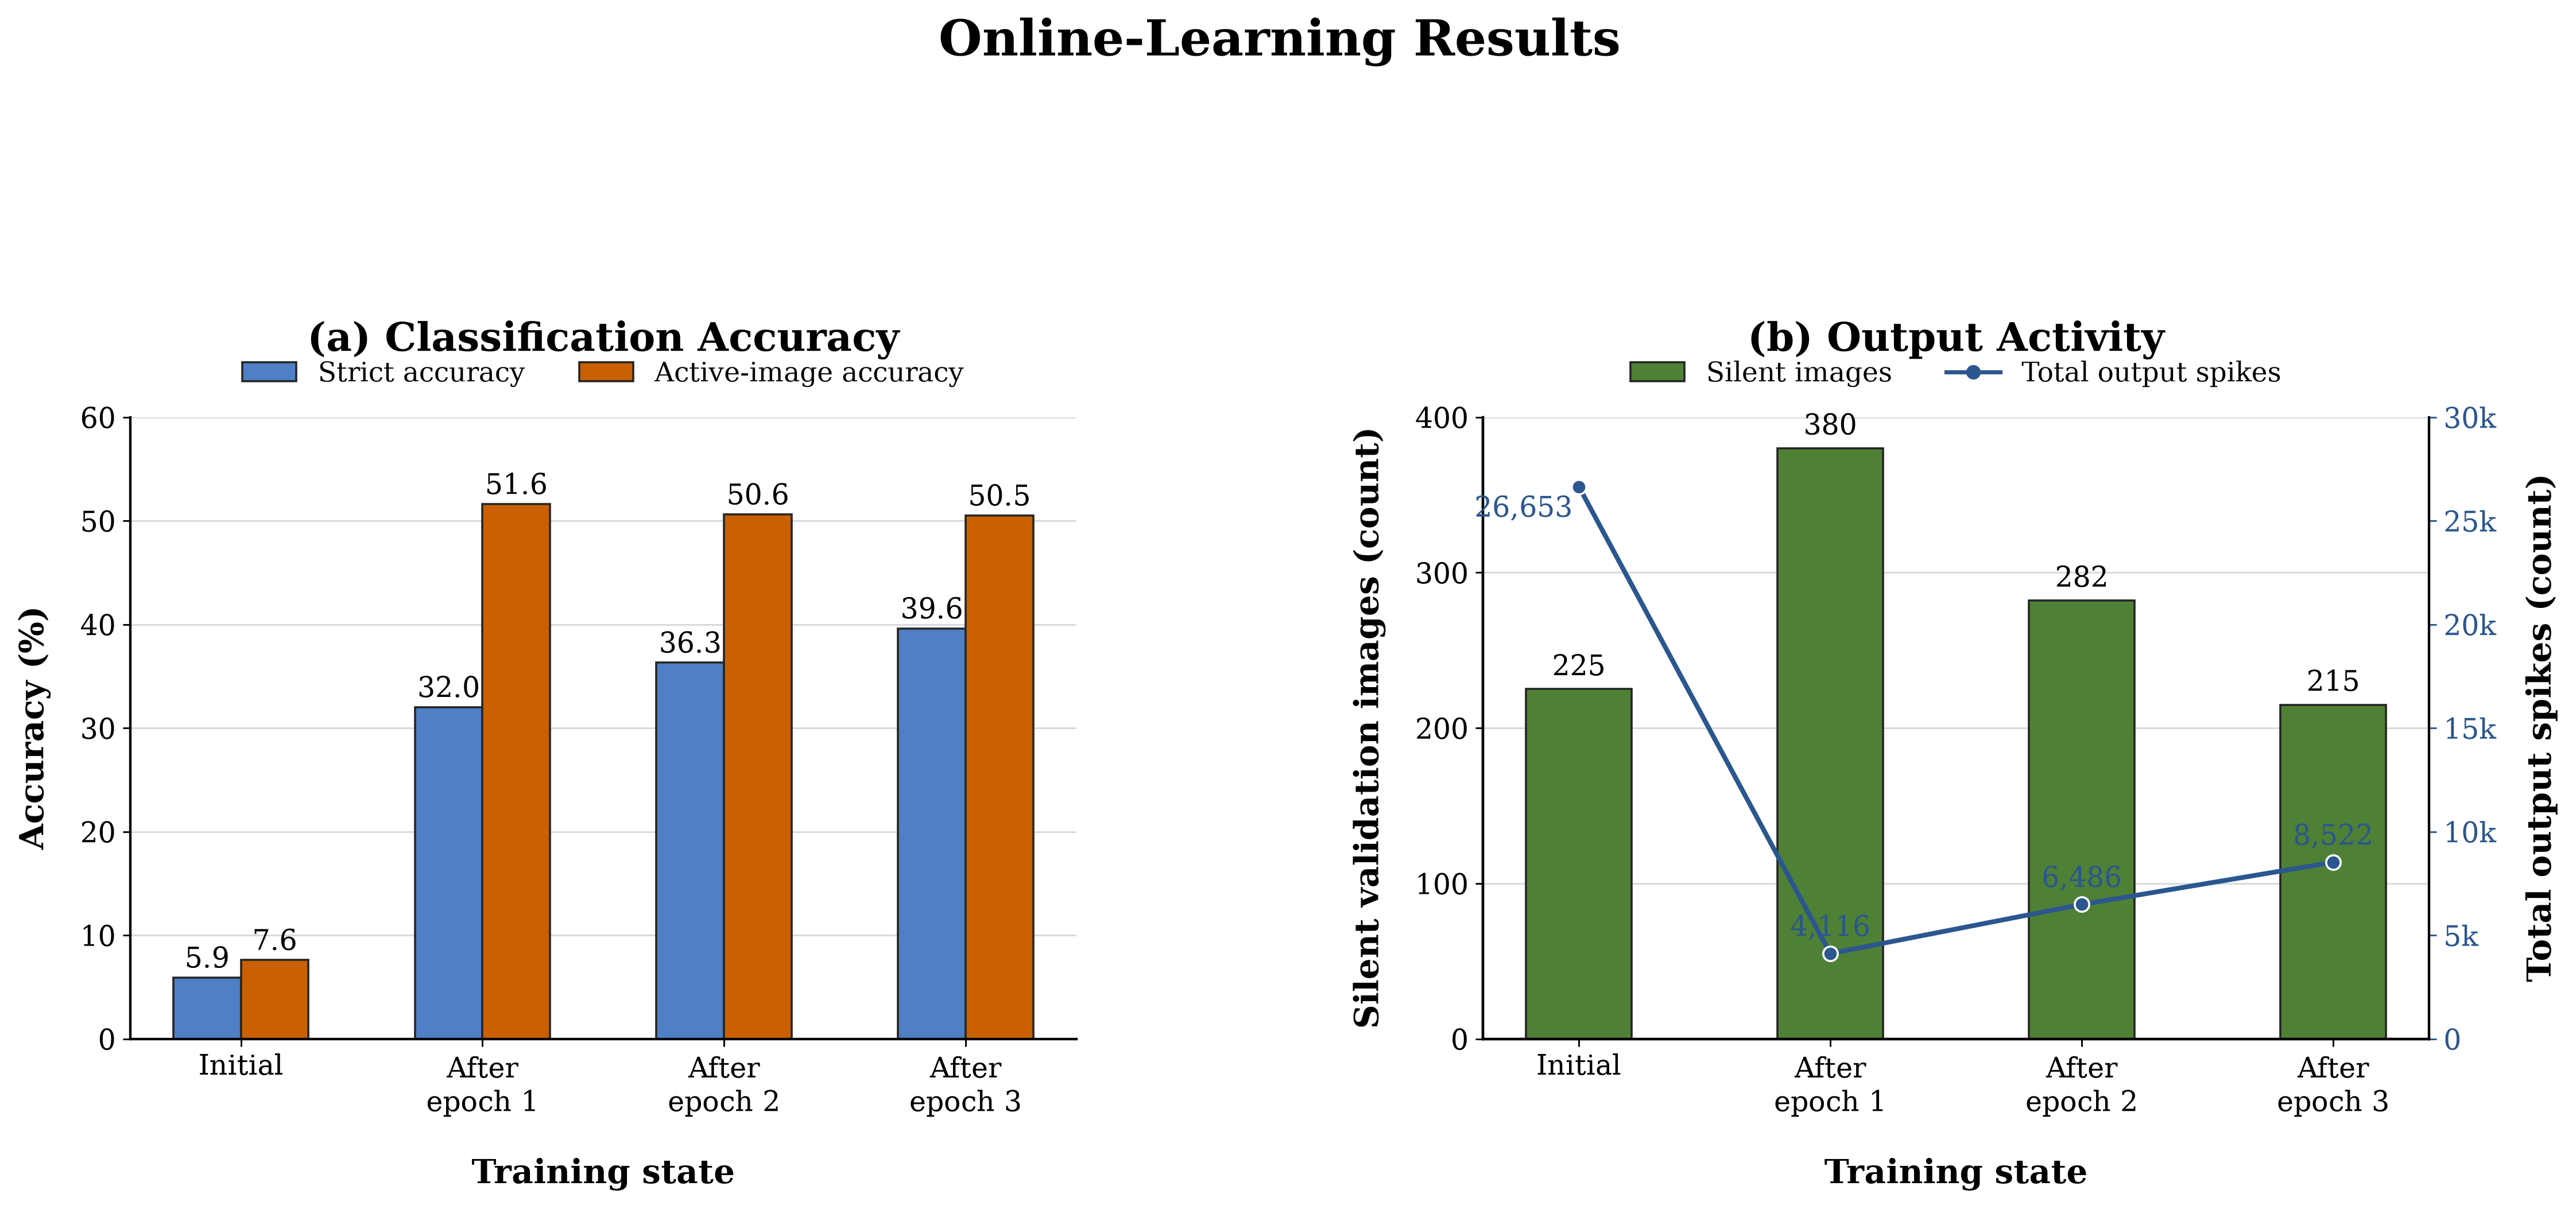
\includegraphics[width=\linewidth]{figures/learning_results_overview.png}
	\caption{Strict and Active-Image Accuracy Together with Output Activity over Three Hardware Training Epochs}
	\label{fig:learning-results-overview}
\end{figure}

The monotonically increasing strict accuracy demonstrates a positive learning trend for the tested configuration. However, the smaller gains in the later epochs and the nearly constant active-image accuracy do not establish convergence. Only one continuous training run was performed, no systematic parameter sweep was carried out, and the accuracy was still increasing after epoch three. The value of 39.6\% should therefore be interpreted as an intermediate validation result after a limited training duration, not as the maximum achievable accuracy of the architecture.

\subsection{Output Activity and Silent Samples}

The activity measurements provide important context for the accuracy curve. The initialized network produces 26,653 output spikes across the validation set, but its strict accuracy is only 5.9\%. High initial activity therefore does not correspond to useful class separation. After the first epoch, the total activity falls to 4,116 spikes and the number of silent images increases from 225 to 380. At the same time, active-image accuracy reaches 51.61\%. The first epoch thus suppresses a large amount of non-discriminative activity while substantially improving the predictions made for images that still produce a response.

During the second and third epochs, output activity partially recovers to 6,486 and 8,522 spikes, while the number of silent images decreases to 282 and then 215. Since active-image accuracy changes only from 51.61\% to 50.45\% across the three trained states, the later increase in strict accuracy is mainly caused by improved response coverage: more validation images produce at least one output spike and can therefore receive a meaningful prediction. The third epoch illustrates this effect most clearly. Strict accuracy rises by 3.3 percentage points from epoch two to epoch three, whereas active-image accuracy decreases slightly from 50.56\% to 50.45\%.

These observations show why output activity must be reported together with accuracy. A reduction in total spikes can remove unwanted responses, but excessive suppression creates silent inputs; conversely, increased activity is beneficial only if the resulting spikes support the correct class. The measured trajectory reflects both effects and cannot be described adequately by a single accuracy value.

\subsection{Per-Class Performance}

Figure~\ref{fig:per-class-learning-accuracy} presents the strict accuracy of each digit class. Because the validation set contains exactly 100 images from every class, each displayed percentage also equals the number of correct images for that class. The results reveal considerable class-dependent variation that is hidden by the aggregate accuracy.

\begin{figure}[t]
	\centering
	\makebox[\linewidth][c]{%
		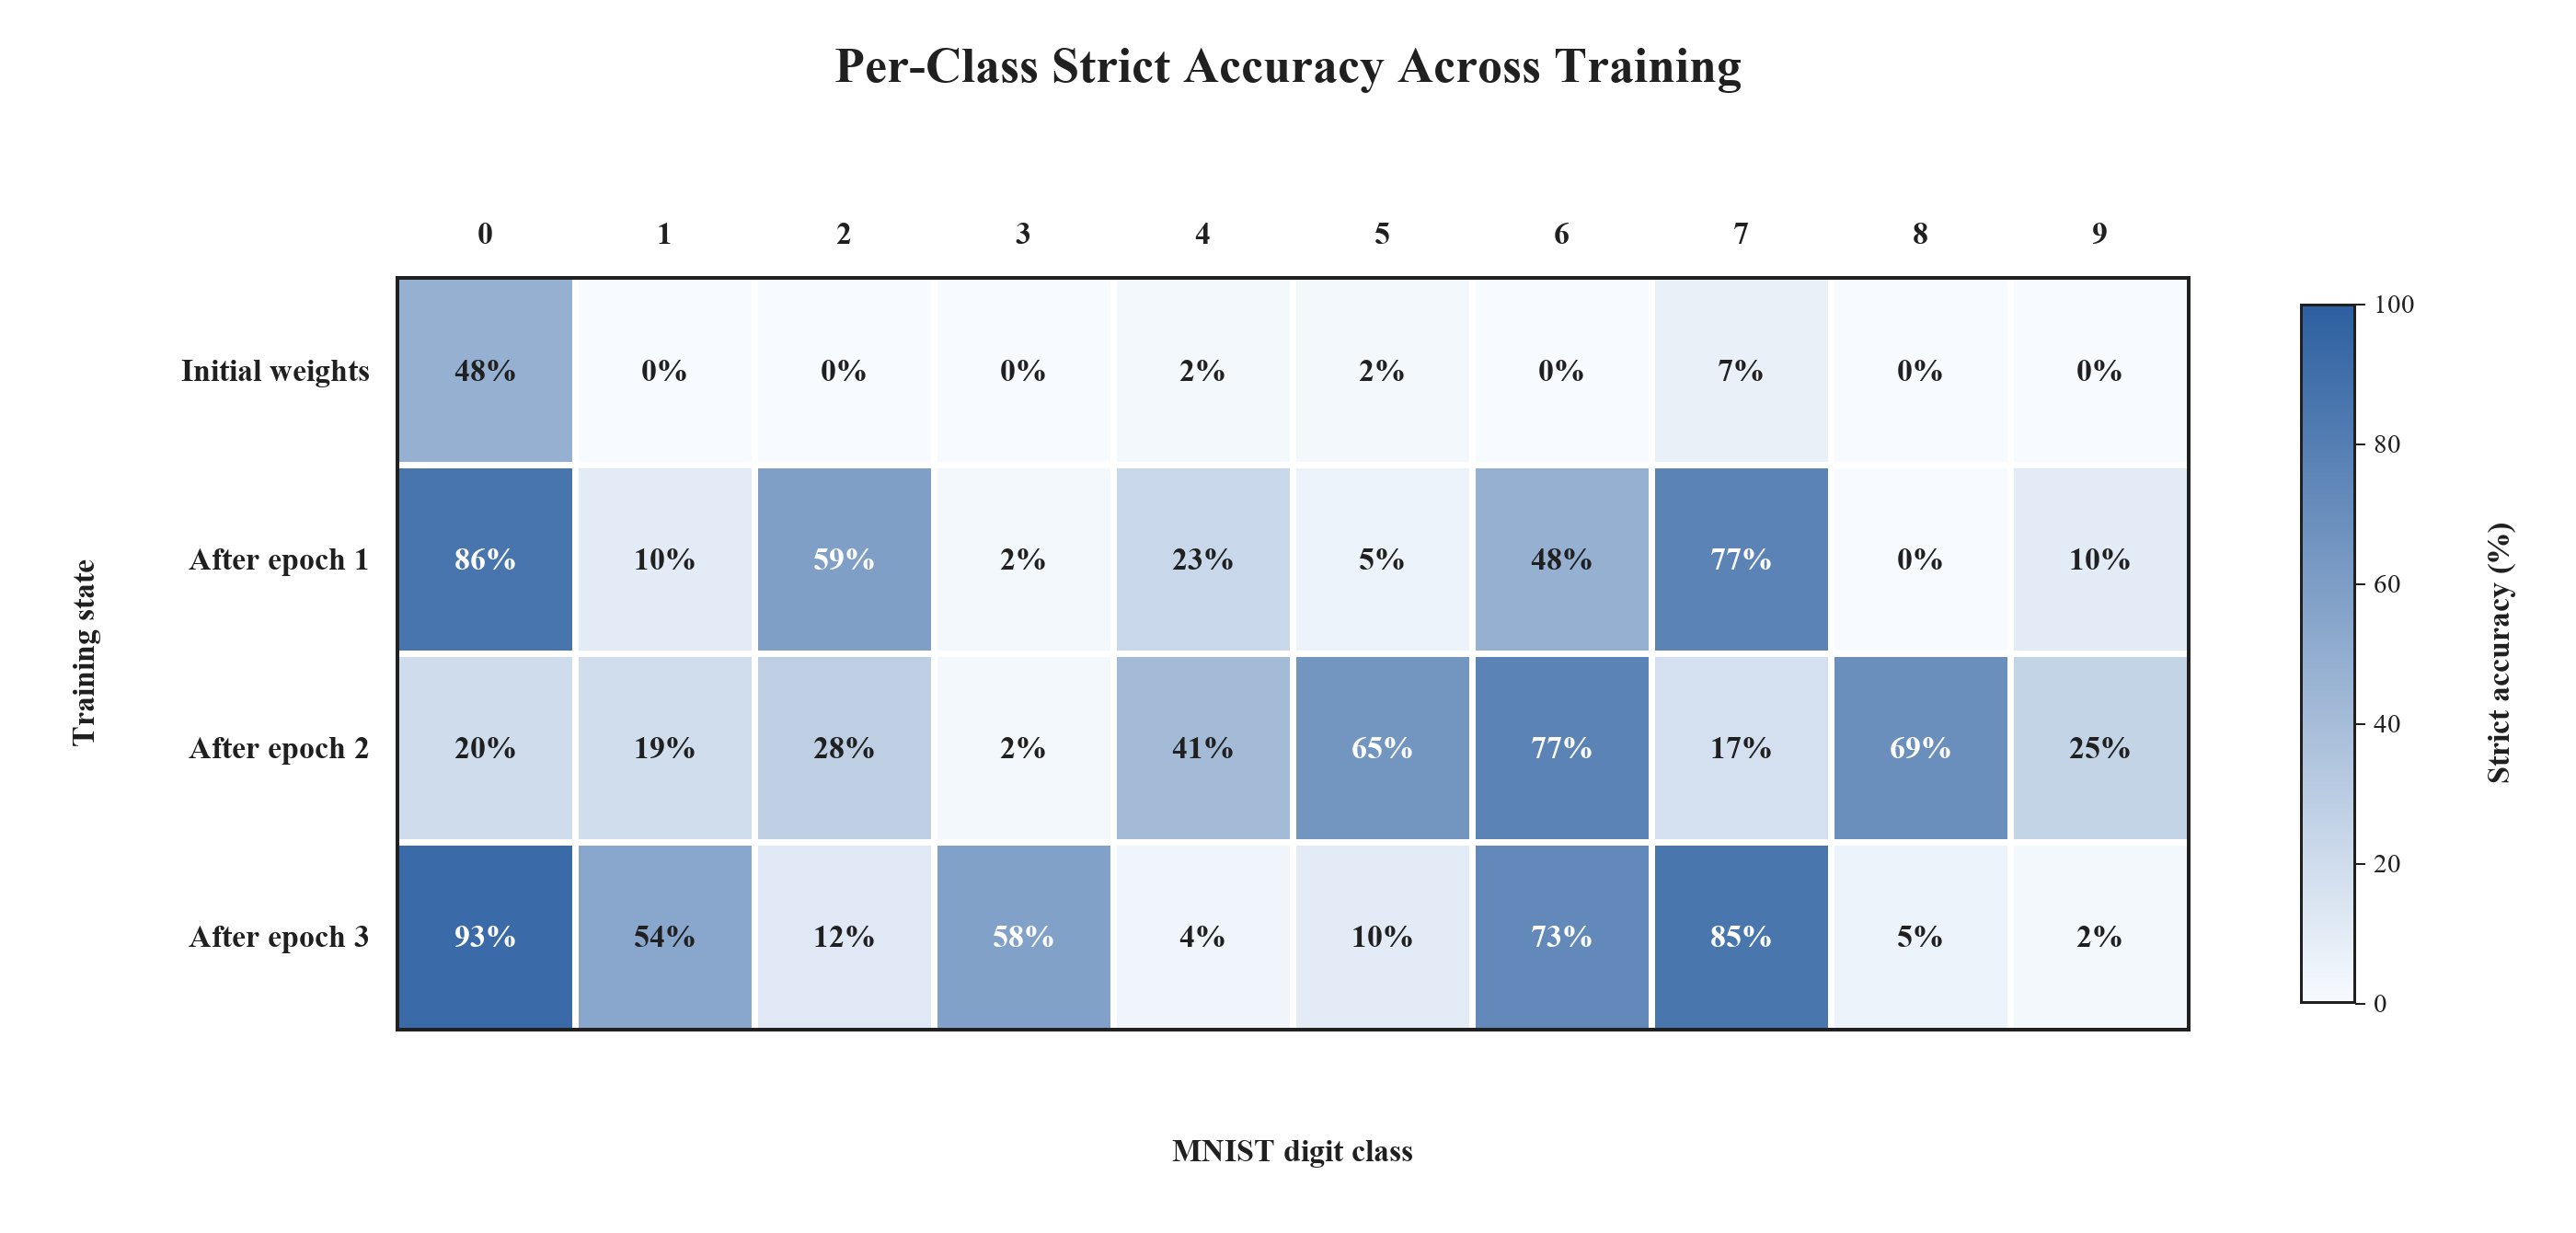
\includegraphics[width=1.06\linewidth]{figures/per_class_learning_accuracy.png}%
	}
	\caption{Per-Class Strict Accuracy on the Fixed Class-Balanced Validation Set}
	\label{fig:per-class-learning-accuracy}
\end{figure}

After the first epoch, classes zero, seven, two, and six achieve the strongest results, with accuracies of 86\%, 77\%, 59\%, and 48\%, respectively. The distribution changes substantially after the second epoch: classes six, eight, and five reach 77\%, 69\%, and 65\%, while the accuracy of classes zero and seven falls to 20\% and 17\%. After the third epoch, classes zero and seven recover to 93\% and 85\%, and classes six, three, and one reach 73\%, 58\%, and 54\%. In contrast, the final accuracies for classes four, eight, and nine are only 4\%, 5\%, and 2\%.

The weak final classes do not all fail in the same manner. For example, 48 of the class-four images and 32 of the class-nine images are silent after epoch three, whereas only 11 class-eight images are silent. The low class-eight accuracy is therefore primarily associated with incorrect competition among active outputs rather than a lack of output activity. This distinction suggests that reducing the overall number of silent samples alone would not remove the observed class imbalance.

The large changes between epochs show that individual class responses had not stabilized within the three-epoch experiment. They may be influenced by the local SDSP dynamics, the discrete 3-bit weight states, the initial weight distribution, and the fixed teacher and calcium parameters, but the present measurements do not isolate the contribution of each factor. The per-class results therefore support the same conclusion as the aggregate curve: the FPGA implements effective online adaptation, but the selected network and training configuration require further epochs and parameter investigation before their classification performance can be considered optimized.

\section{Comparison with SDSP-Based Related Work}
\label{subsec:comparison-with-related-work}

The broad literature review in Table~\ref{tab:related-work-comparison} includes both \gls{sdsp}- and \gls{stdp}-based systems. For evaluation of the implemented learning architecture, the comparison is narrowed to ODIN, MorphIC, the multiplier-less \gls{sdsp} circuit of Asgari et al., and TEDOP \cite{Frenkel2019ODIN,Frenkel2019MorphIC,Asgari2020SDSP,Shi2022TEDOP}. These works all implement \gls{sdsp} or a directly derived stochastic variant, but they differ substantially in technology, neuron dynamics, topology, input preparation, and evaluation scope. The values below therefore position the present design within this family of approaches; they do not form a normalized ranking.

\subsection{Rationale for the Single-Layer Network}

The 784--10 topology used in this work was selected deliberately to match the input and output dimensions of the MNIST network evaluated by TEDOP \cite{Shi2022TEDOP}. Using no hidden layer keeps the principal comparison focused on the integration of online synaptic plasticity into an event-driven hardware datapath. Introducing a hidden layer could improve the representational capacity of the classifier, but it would also change the synaptic memory, processing schedule, and learning dynamics. The resulting system would consequently be less useful as a structural reference to TEDOP.

This choice should not be interpreted as an assertion that a single-layer network is optimal for MNIST. Its purpose is methodological: it provides a compact and reproducible configuration in which weight write-back, teacher guidance, and persistent online adaptation can be evaluated on the \gls{fpga}. ODIN also evaluates a single-layer ten-class classifier, but its input is reduced to 256 values; MorphIC and the circuit of Asgari et al. do not provide an equivalent 784--10 online-learning experiment. TEDOP is therefore the closest topological reference, even though it is not algorithmically identical to the present network.

\subsection{Algorithmic Context}

Among the selected systems, ODIN is the closest reference for the learning rule itself. Its teacher-supervised \gls{sdsp} decision uses a presynaptic event together with the postsynaptic membrane potential and calcium state, as does the implementation developed in this thesis \cite{Frenkel2019ODIN}. However, ODIN embeds the rule in a time-multiplexed custom processor with configurable neuron dynamics and a $(3+1)$-bit synapse format. MorphIC instead adapts \gls{sdsp} to binary weights by applying eligible transitions stochastically. Its online demonstration is an eight-pattern task, whereas its 97.8\% MNIST result uses weights trained offline \cite{Frenkel2019MorphIC}. The design by Asgari et al. uses a 32-bit fixed-point state and demonstrates potentiation and depression in a two-neuron, one-synapse network, but it does not report a classification experiment \cite{Asgari2020SDSP}.

TEDOP uses a 16-bit Temporal-Integrate neuron derived from the integrate-and-fire model by removing its firing mechanism \cite{Shi2022TEDOP}. Its membrane potential is updated only when an input event is received. Each event contributes the corresponding excitatory weight minus a constant inhibitory term, while an additional teacher term may be applied during training. The neuron has no firing threshold, produces no output spikes, and performs no firing reset. After all events belonging to a sample have been processed, the decision unit selects the neuron with the largest final membrane potential.

The associated S4DSP rule also differs from the calcium-dependent \gls{sdsp} implementation used in this thesis. TEDOP evaluates the membrane potential against three update thresholds and probabilistically increments or decrements the active synaptic weight. The random decision is generated by a linear-feedback shift register. By exploiting an approximate relationship between the accumulated Temporal-Integrate potential and the output-spike count of a reference integrate-and-fire neuron, S4DSP removes the separate calcium state used by conventional \gls{sdsp}. This co-simplification of the neuron and learning models is central to TEDOP's small hardware footprint \cite{Shi2022TEDOP}.

In contrast, the present accelerator retains the modified subtractive-reset \gls{lif} neurons generated by Spiker+, including output-spike generation, reset behaviour, and recurrent output inhibition. Classification is based on the ten output spike counts rather than on final membrane potentials. The implemented \gls{sdsp} rule stores a calcium counter for each postsynaptic neuron and combines its state with the membrane-potential condition to form the \texttt{up} and \texttt{down} decisions. The selected 3-bit weight is then changed by one discrete level with saturation. Consequently, the equal 784--10 dimensions provide a useful topological reference to TEDOP, but they do not make the two classifiers equivalent.

\subsection{Quantitative Comparison and Measurement Boundaries}

Table~\ref{tab:sdsp-evaluation-comparison} repeats the \gls{sdsp}-based references from Chapter~\ref{sec:related_work}, adds the present implementation, and includes the quantitative implementation data that are relevant only after the measurement methodology of this chapter has been established. Values for the present work are those reported in the preceding sections.

% Quantitative comparison for Section 6.6.
\begin{table}[p]
	\centering
	\caption{Comparison with SDSP-Based Related Work}
	\label{tab:sdsp-evaluation-comparison}
	\begingroup
	\scriptsize
	\sloppy
	\setlength{\tabcolsep}{1.8pt}
	\renewcommand{\arraystretch}{1.03}
	\begin{tabularx}{\textwidth}{@{}
		>{\raggedright\arraybackslash}p{1.45cm}
		*{5}{>{\raggedright\arraybackslash}X}@{}}
		\toprule
		\textbf{Metric} &
		\shortstack[l]{\textbf{ODIN}\\\cite{Frenkel2019ODIN}} &
		\shortstack[l]{\textbf{MorphIC}\\\cite{Frenkel2019MorphIC}} &
		\shortstack[l]{\textbf{Asgari et al.}\\\cite{Asgari2020SDSP}} &
		\shortstack[l]{\textbf{TEDOP}\\\cite{Shi2022TEDOP}} &
		\textbf{This work} \\
		\midrule

		\textbf{Platform} &
		28-nm ASIC &
		65-nm ASIC &
		Spartan-6 XC6SLX45 FPGA &
		Zynq-7010 FPGA &
		PYNQ-Z1, XC7Z020 FPGA \\

		\textbf{Evaluated boundary} &
		Complete neuromorphic chip &
		Complete four-core chip &
		Two-neuron, one-synapse test network &
		Specialized learning core &
		Complete PL design; PS included in power estimate \\

		\textbf{Topology} &
		256--10 MNIST classifier &
		Four-core hierarchy; eight-class online benchmark &
		1--1 test network &
		784--10 MNIST classifier &
		784--10 MNIST classifier \\

		\textbf{Neuron and decision} &
		Configurable LIF or phenomenological neuron; rate or first-spike decision &
		LIF neurons; task-dependent output aggregation &
		LIF neurons with a calcium estimator &
		16-bit Temporal-Integrate; final-potential argmax &
		Modified subtractive-reset LIF; output-spike-count argmax \\

		\textbf{Learning and weights} &
		Teacher-supervised SDSP; 3-bit weight plus mapping bit &
		Stochastic SDSP; binary weights &
		Multiplier-less SDSP; 32-bit fixed point &
		Stochastic S4DSP; 8-bit weights &
		Calcium- and membrane-dependent SDSP; 3-bit weights \\

		\textbf{Input and training protocol} &
		28$\times$28 to 16$\times$16, deskewed and soft-thresholded; 6k samples presented once &
		Online eight-pattern task; reported MNIST result uses offline training &
		Synthetic spike trains; no classifier training &
		784-pixel rate code; 200 steps; epoch count N/R &
		784-pixel rate code; 100 steps; three 60k-sample epochs \\

		\textbf{Clock} &
		75~MHz &
		55~MHz &
		131~MHz &
		250~MHz &
		100~MHz \\

		\textbf{Reported implementation} &
		0.086\,$\mathrm{mm}^{2}$; 256 neurons; 64k synapses &
		2.86\,$\mathrm{mm}^{2}$; ${\sim}$2k neurons; ${>}$2M synapses &
		450 LUTs; 249 registers &
		952 LUTs; 741 FFs; 4 BRAMs; 0 DSPs &
		5,056 LUTs; 5,294 FFs; 4 BRAMs \\

		\textbf{Power or energy} &
		12.7~pJ/SOP; 15~nJ/inference at 0.55~V &
		51~pJ/SOP; 21.8~$\mu$J/classification &
		N/R &
		39~mW; 3.46~$\mu$J/training image; 3.32~$\mu$J/inference image &
		1.445~W whole-device estimate; isolated energy N/R \\

		\textbf{Online-learning result} &
		85.0\% rate; 84.5\% rank order on full 10k MNIST test set &
		800/800 pattern samples; 97.8\% MNIST is offline &
		LTP and LTD verified; no classification result &
		90.4\% MNIST test accuracy &
		39.6\% strict accuracy on fixed 1k validation set after epoch three \\

		\textbf{Reported rate} &
		N/R &
		N/R &
		N/A &
		11,268 training; 11,749 inference frames/s &
		66.16 training; ${\sim}$67.8 inference images/s end-to-end \\
		\bottomrule
	\end{tabularx}
	\endgroup
\end{table}


The implementation values describe different technologies and boundaries. ODIN and MorphIC report fabricated \gls{asic} area and capacity, which cannot be converted directly into \gls{fpga} logic utilization. The Asgari result covers only a minimal test network, and TEDOP reports a specialized neuromorphic core. By contrast, the values for this work cover the complete programmable-logic design, including the accelerator IP, AXI control, \gls{dma}, interconnect, and buffering infrastructure. The larger LUT and flip-flop totals therefore do not quantify the incremental cost of the \gls{sdsp} block alone.

The power and energy values are also unsuitable for a direct ranking. ODIN and MorphIC report operation- or classification-level energy for custom chips, while TEDOP reports prototype power and derived energy per image. The 1.445~W value for this work is a medium-confidence Vivado estimate for the complete Zynq device and is dominated by 1.260~W attributed to the PS7; no isolated accelerator energy was measured. Similarly, the 66--68 images/s measured here include Python control, buffer management, \gls{dma} transfers, register access, status polling, and an explicit 10~ms software delay per image. TEDOP's 11,268 training frames/s and 11,749 inference frames/s describe its specialized 250~MHz processing path \cite{Shi2022TEDOP}. The reported differences therefore characterize complete evaluation setups rather than equivalent learning datapaths.

\subsection{Interpretation of the Learning Results}

The accuracy values require the same separation of experimental conditions. ODIN reports 85.0\% rate-coded and 84.5\% rank-order accuracy after presenting 6,000 training samples once and evaluating the full 10,000-image MNIST test set \cite{Frenkel2019ODIN}. Before encoding, however, its images are compressed from $28\times28$ to $16\times16$, deskewed, and soft-thresholded. The present work instead retains 784 image inputs and uses the Spiker+ rate encoder for 100 time steps. ODIN's result is therefore evidence that single-layer \gls{sdsp} can perform substantially better under a different input and decision pipeline, not a controlled comparison of the learning circuit alone.

MorphIC's 97.8\% MNIST figure should not be compared with the online-learning curve because it is obtained with offline quantization-aware training; its online result is the separate eight-pattern experiment \cite{Frenkel2019MorphIC}. Likewise, Asgari et al. verify individual long-term potentiation and depression responses but do not report classification accuracy \cite{Asgari2020SDSP}. Keeping these distinctions in the table prevents an offline result or a circuit-level verification from being interpreted as an online MNIST benchmark.

TEDOP achieves 90.4\% MNIST test accuracy, whereas the present hardware reaches 39.6\% strict accuracy on the fixed validation set after three epochs. Several coupled differences can contribute to this gap. TEDOP uses 8-bit weights, a 16-bit non-spiking Temporal-Integrate state, 200 rate-coded time steps, final-potential classification, and stochastic potential-dependent S4DSP. This work uses 3-bit weights, spiking \gls{lif} neurons with recurrent inhibition, 100 time steps, spike-count classification, and an explicit calcium state. TEDOP does not state the number of training epochs, while the present experiment uses one run with one fixed parameter set. The two accuracy values consequently compare complete classifier configurations rather than isolated learning rules.

The learning curve in Figure~\ref{fig:learning-results-overview} was still increasing after the third epoch, and the per-class responses had not stabilized. The measured 39.6\% should therefore be treated as an intermediate result rather than a convergence value. Training beyond five epochs, parameter tuning, and repeated runs are required before the attainable accuracy can be assessed. At the same time, the current result cannot be explained only by insufficient training: ODIN reaches its reported result with fewer sample presentations but uses different preprocessing, encoding, neuron dynamics, and inference criteria. These comparisons identify the input pipeline and the coupled neuron--learning configuration as important evaluation variables for future experiments.

The comparison consequently supports a narrower conclusion than an accuracy ranking. ODIN and MorphIC demonstrate alternative custom-chip realizations of state-dependent learning, Asgari et al. provide a detailed high-resolution circuit reference, and TEDOP demonstrates the performance obtainable from a highly specialized joint neuron--learning architecture. The contribution of the present work is the integration and board-level validation of persistent \gls{sdsp} weight updates within the reusable Spiker+ architecture and its PYNQ deployment path. Matching TEDOP's single-layer topology makes that distinction explicit while preserving a meaningful external reference for the measured results.

\section{Discussion and Limitations}
\label{subsec:discussion-and-limitations}

The results demonstrate that the main architectural objective of this work was achieved: an accelerator generated by Spiker+ was extended with a synthesizable \gls{sdsp} learning path, writable synaptic memory, and the control required to retain updated weights during operation. The contribution should nevertheless be evaluated at two different levels. At the hardware level, the experiments provide strong evidence for correct integration and continuous operation. At the application level, they demonstrate online adaptation but not a converged or optimized MNIST classifier. Table~\ref{tab:evaluation-evidence-and-limitations} summarizes these claim boundaries.

\begin{table}[htbp]
	\centering
	\caption{Evaluation Evidence, Supported Conclusions, and Remaining Limitations}
	\label{tab:evaluation-evidence-and-limitations}
	\small
	\begin{tabularx}{\linewidth}{@{}p{0.16\linewidth}p{0.25\linewidth}X X@{}}
		\toprule
		\textbf{Aspect} & \textbf{Evidence} & \textbf{Supported conclusion} & \textbf{Not established} \\
		\midrule
		Weight update & Teacher-on/off control and restoration after bitstream reload & Supervised operation produces a persistent, target-dependent change & Direct values of every modified synapse \\
		System integration & Interface tests and 180,000 completed training transactions & The PS, DMA, accelerator, and learning path operate continuously as an integrated system & Behaviour on other boards or with other network and interface configurations \\
		Implementation & Timing closure at 100~MHz and low device utilization & The complete design is deployable on the PYNQ-Z1 with resource headroom & Maximum frequency and network-scaling limits \\
		Online learning & Strict accuracy increases from 5.9\% to 39.6\% over three epochs & The implemented local updates improve classification for the tested configuration & Convergence, optimized accuracy, or statistical variation across runs \\
		Performance & Stable end-to-end training and inference times & The deployed application provides repeatable transaction-level operation & Isolated core throughput, measured energy per image, or normalized superiority over TEDOP \\
		\bottomrule
	\end{tabularx}
\end{table}


\subsection{Assessment of the Implemented Contributions}

The controlled teacher experiment provides the clearest evidence for persistent learning. Enabling the teacher path changed later inference results only after supervised training, the changes were confined to the selected output neuron, and reloading the bitstream restored the initial response. Together with the RTL verification described in Chapter~\ref{sec:implementation}, these observations support the conclusion that the implemented read--modify--write path updates synaptic state and that the updated value affects subsequent input transactions. Because the complete weight memory is not exposed to the processor, this conclusion is based on controlled behavioural evidence rather than direct read-back of every modified weight.

The system-level tests also show that the learning extension was successfully integrated into the PYNQ deployment path. The design accepted the zero-input, dense-input, fixed MNIST, and supervised-training transactions without a stream error or incomplete input count. It then processed 180,000 training images across three continuous epochs without reconfiguration. The implemented design meets timing at 100~MHz and occupies less than 10\% of the available LUTs and less than 5\% of the flip-flops on the XC7Z020. These results establish feasibility on the target platform and leave resource headroom for future extensions. They do not, however, determine the maximum clock frequency or the largest network that can be supported, because neither frequency scaling nor network-size scaling was evaluated.

The inference-only operating mode was retained. When learning and teacher input were disabled, the same accelerator processed validation samples without issuing new weight writes. This runtime selection satisfies the design requirement that the learning extension should not require a separate bitstream for inference. The comparison with the Spiker+ software model further showed similar baseline activity after the RTL initial weights had been aligned, although the two implementations were not bit-exact because they use different numerical representations and execution schedules.

\subsection{Interpretation of the Learning Behaviour}

The increase in strict accuracy from 5.9\% to 39.6\% demonstrates that the local hardware updates produce a useful change at the network level. The result is particularly relevant because the evaluation was performed with learning and teacher input disabled. The measured improvement therefore reflects the retained weight state rather than a direct contribution from the teacher current during classification. The positive trend across all three epochs additionally shows that the first improvement was not an isolated short-term training effect.

The activity results also reveal why this improvement must be interpreted cautiously. The first epoch removes a large amount of initially non-discriminative spiking, but it also increases the number of silent samples. Later epochs restore response coverage and improve strict accuracy, while active-image accuracy remains close to 50\%. The network is therefore learning both when to respond and which class should win, and these two effects progress at different rates. The large changes in class-wise accuracy between epochs further show that the output competition had not stabilized.

Several design choices restrict the attainable result of the evaluated configuration. The single-layer topology has limited representational capacity, the 3-bit weights allow only eight synaptic states, and the 100-step input window limits the available temporal evidence. The selected teacher current, calcium-leak interval, neuron parameters, and input gain were kept fixed, while bistability was disabled. These factors may influence the silent-sample rate, competition between output neurons, and the balance between potentiation and depression. The present experiment did not vary them independently, so none of them can be identified as the sole cause of the observed class imbalance.

Most importantly, the three-epoch experiment ended while strict accuracy was still increasing. It therefore does not establish convergence or the maximum accuracy of the architecture. A convergence study should extend training beyond five epochs and evaluate intermediate checkpoints using an independent test set. Parameter tuning should be performed separately from the final assessment and should consider at least the teacher strength, calcium thresholds and leakage, neuron threshold, rate-coding gain, input duration, and the optional bistability mechanism. Repeated runs would then be required to distinguish systematic improvement from variation caused by weight initialization, sample order, and stochastic spike encoding.

\subsection{Limitations of the Experimental Evidence}

The first limitation is statistical. Only one continuous training run was performed, using one initial weight state and three predetermined spike-generation seeds. Although the validation inputs were held fixed and the complete training archives were recorded for reproducibility, the experiment provides no variance or confidence interval across independent runs. The observed learning curve is consequently evidence for the behaviour of the evaluated configuration, not an estimate of its expected performance over random initial conditions.

The second limitation concerns dataset usage. The 1,000 class-balanced images were taken from the MNIST test partition, but their results were inspected after every epoch and used when deciding whether to continue training. They therefore function as a validation set rather than an untouched final test set. Reporting the 39.6\% value as final test accuracy would overstate the strength of the evaluation. A future experiment should use separate training, validation, and test partitions, with the test set evaluated only after the training duration and parameters have been fixed.

The third limitation is observability. The processor interface exposes accepted-step counts, status information, and output-neuron spike counts, but it does not provide direct access to every online weight value or internal calcium state. The teacher-control experiment and the restoration after bitstream reload provide consistent evidence of persistent updates, yet they cannot replace a complete trace of individual synaptic transitions. Adding a debug-only weight read-back interface or an internal logic-analyser configuration would enable a more direct board-level comparison with the expected \gls{sdsp} update sequence.

Finally, the comparison in Section~\ref{subsec:comparison-with-related-work} is limited by the absence of a common measurement boundary. No physical board-power measurement, isolated accelerator cycle count, or energy-per-classification measurement was obtained for this work. The available implementation and runtime results are sufficient to demonstrate deployability and stable end-to-end execution, but not to establish a normalized performance or energy advantage over another processor.

Overall, the evaluation validates the hardware contribution more strongly than the classifier performance. The integrated system performs persistent online updates, preserves an inference mode, meets the selected timing constraint, and operates reliably for a complete multi-epoch workload. The measured accuracy confirms useful adaptation, but remains an intermediate result whose convergence, robustness, and parameter sensitivity require additional experiments. This distinction defines the conclusions that can be drawn from the present thesis without extending them beyond the available evidence.
